% Written by: Erick Cobos T
% Date: 24-November-2016

\documentclass{beamer}

\usepackage{subcaption}
\usepackage{verbatim}
\usepackage[utf8]{inputenc}


% To add sources at end
\newcommand{\source}[1]{\vskip0pt plus 1filll \scriptsize #1}

% Theme config
\usetheme{Madrid}
\usecolortheme{seahorse} %beaver for red, seahorse for blue


% Title information
\title[Thesis Dissertation]{Segmentation of Breast Cancer Masses in Digital Mammograms: A Convolutional Network}
\subtitle{Master's thesis}
\author[Erick Cobos]{Erick Cobos Tandazo \\ \medskip \footnotesize \textbf{Advisor:}\\Dr. Hugo Terashima Marín \\ \textbf{Supervisors:}\\Dr. Santiago Enrique Conant Pablos\hfill Dr. José Gerardo Tamez Peña}
\date[December, 2016]{December, 2016}
\institute[Tec de Monterrey]{
    Centro de Sistemas Intelligentes \\ Tecnologico de Monterrey}
\subject{Machine Learning}


% Put table of contents before every section
\AtBeginSection[]{
  \begin{frame}
    \frametitle{Table of Contents}
    \tableofcontents[currentsection]
  \end{frame}
}

\begin{document}
	\begin{frame}
		\titlepage
		% the objective of this talk is to report the results of my thesis, explain what has been done, the justification to some of the deicisions taken, what are the conclusions reached and what future work could stillbe done.
	\end{frame}
		
    \section[Introduction]{Introduction}
    \begin{frame}
		\frametitle{Thesis objective}
			The main goal is to segment breast cancer lesions using convolutional networks, an end-to-end learnable model.
		
		\begin{itemize}
			\item Obtain and process the mammographic database. %to make it available for future research on campus.
			\item Develop software to handle the database and train new deep learning models.
			\item Develop and train modern, fine-tuned convolutional networks.% to perform lesion segmentation.
			\item Test the viability of convolutional networks for breast cancer research through different experiments.
			\item Propose ideas for future research in the area.
		\end{itemize}
	\end{frame}
   
    \section[Breast Cancer]{Breast Cancer}
    \begin{frame}
     	\frametitle{Why breast cancer?}
     		Breast cancer is the most commonly diagnosed cancer among women.
     		
     		For women, death rates are the second highest of any cancer. However, survival rate when detected early is close to 100\%.
     		
     		On-going project at the institution.
    \end{frame}
%Cancer es un término que se usa para describir varias enfermedades distintas donde celulas anomalas se dividen sin control produciendo tuimores y eventualmente invadiendo tejido cercano. Breast cancer es cuando se genera en tejidos del seno.
%Besides skin cancer, breast cancer is one of the most commonly diagnosed cancer among American women.  Just under 30% of cancers in women are breast cancers. 
%About 1 in 8 U.S., UK women will develop invasive breast cancer.
%Death rates higher than those for any other cancer, besides lung cancer.
%People in the campus have been wporking on this already.

	\begin{frame}
		\frametitle{Breast cancer signs}
		Masses vs. microcalcifications
		\begin{figure}[h]
			\centering
			\begin{subfigure}{0.35\textwidth}
				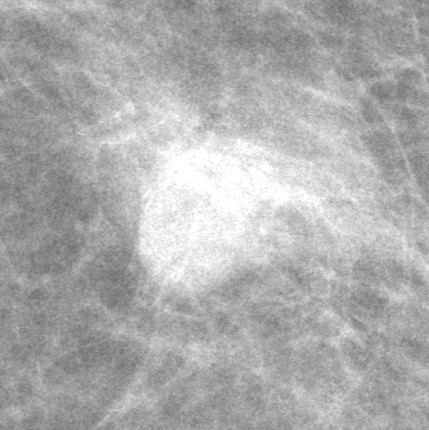
\includegraphics[width=\textwidth]{plots/breastMass.jpg}
			\end{subfigure}
			~
			\begin{subfigure}{0.35\textwidth}
				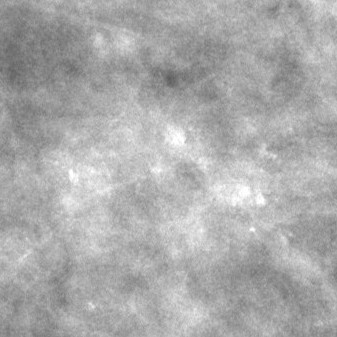
\includegraphics[width=\textwidth]{plots/breastMicrocalcification.jpg}
			\end{subfigure}
		\end{figure}

		Detection vs. diagnosis
	\end{frame}
% Mammography is the main tool. we focus on this and this.
	
	\begin{frame}
		\frametitle{Lesion segmentation}
		\begin{figure}[h]
			\centering
			\begin{subfigure}{0.35\textwidth}
				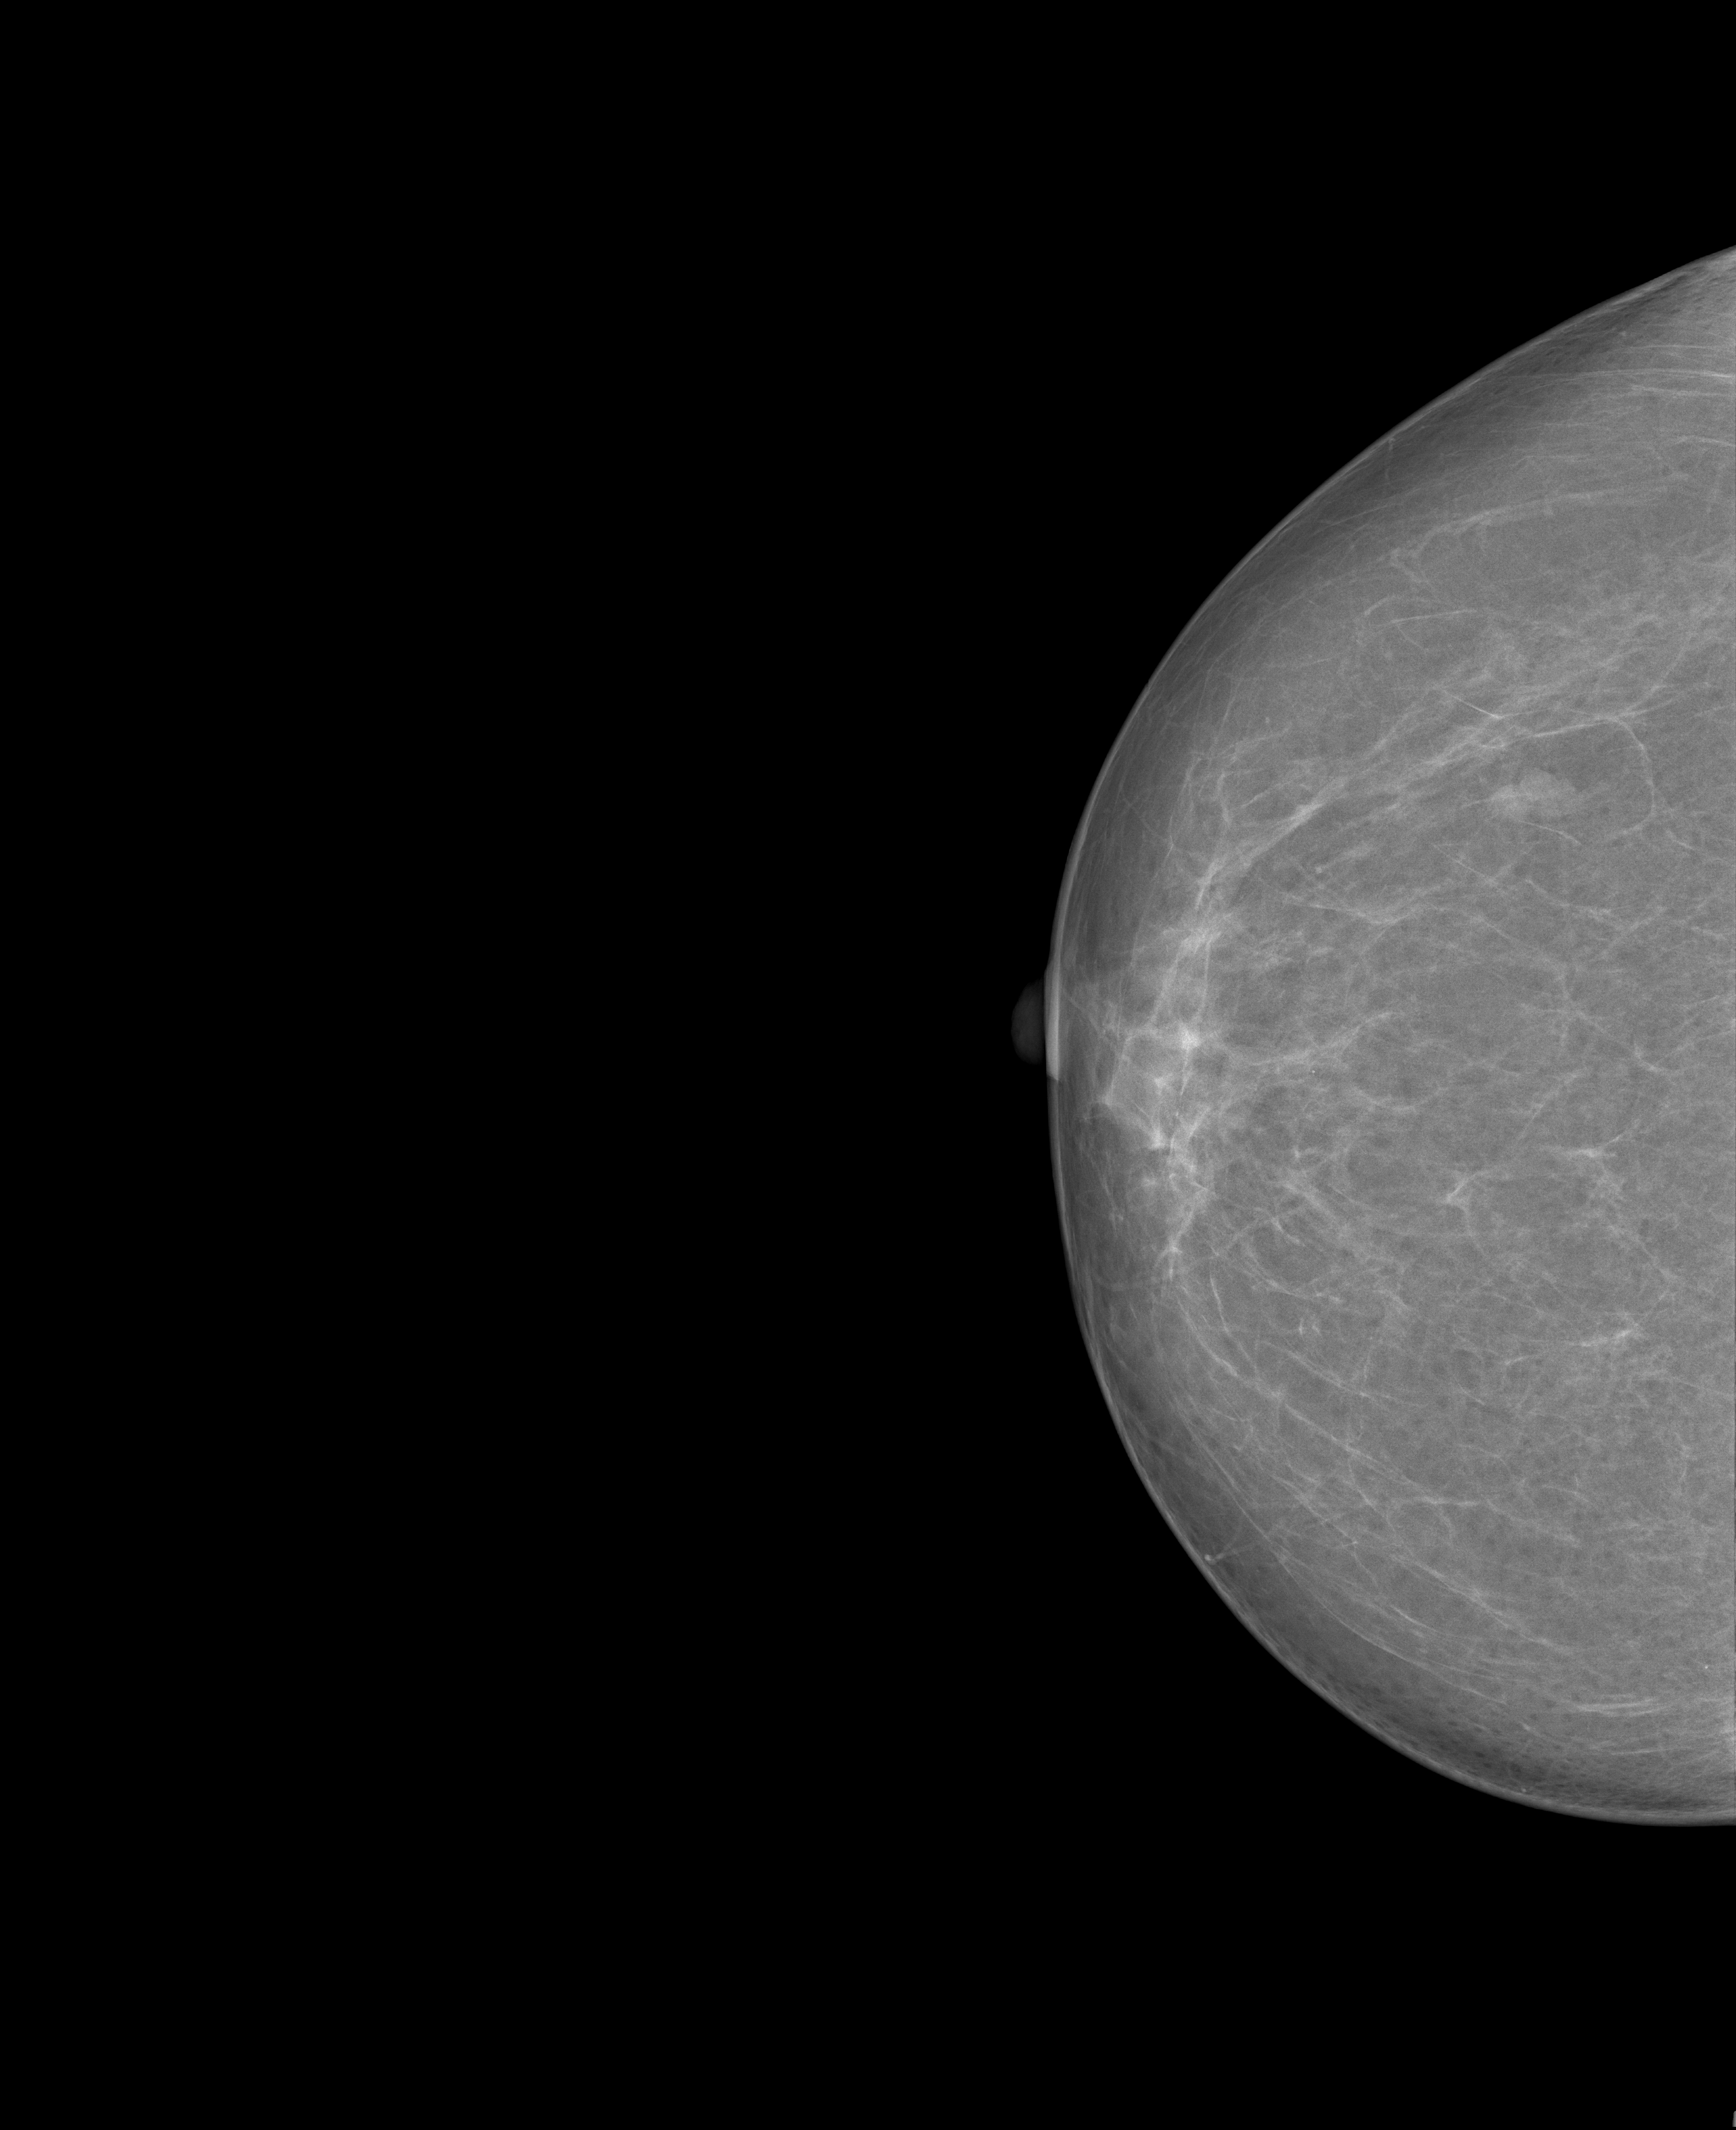
\includegraphics[width=\textwidth]{plots/mammogram.png}
				\caption{Mammogram}
			\end{subfigure}
			~
			\begin{subfigure}{0.35\textwidth}
				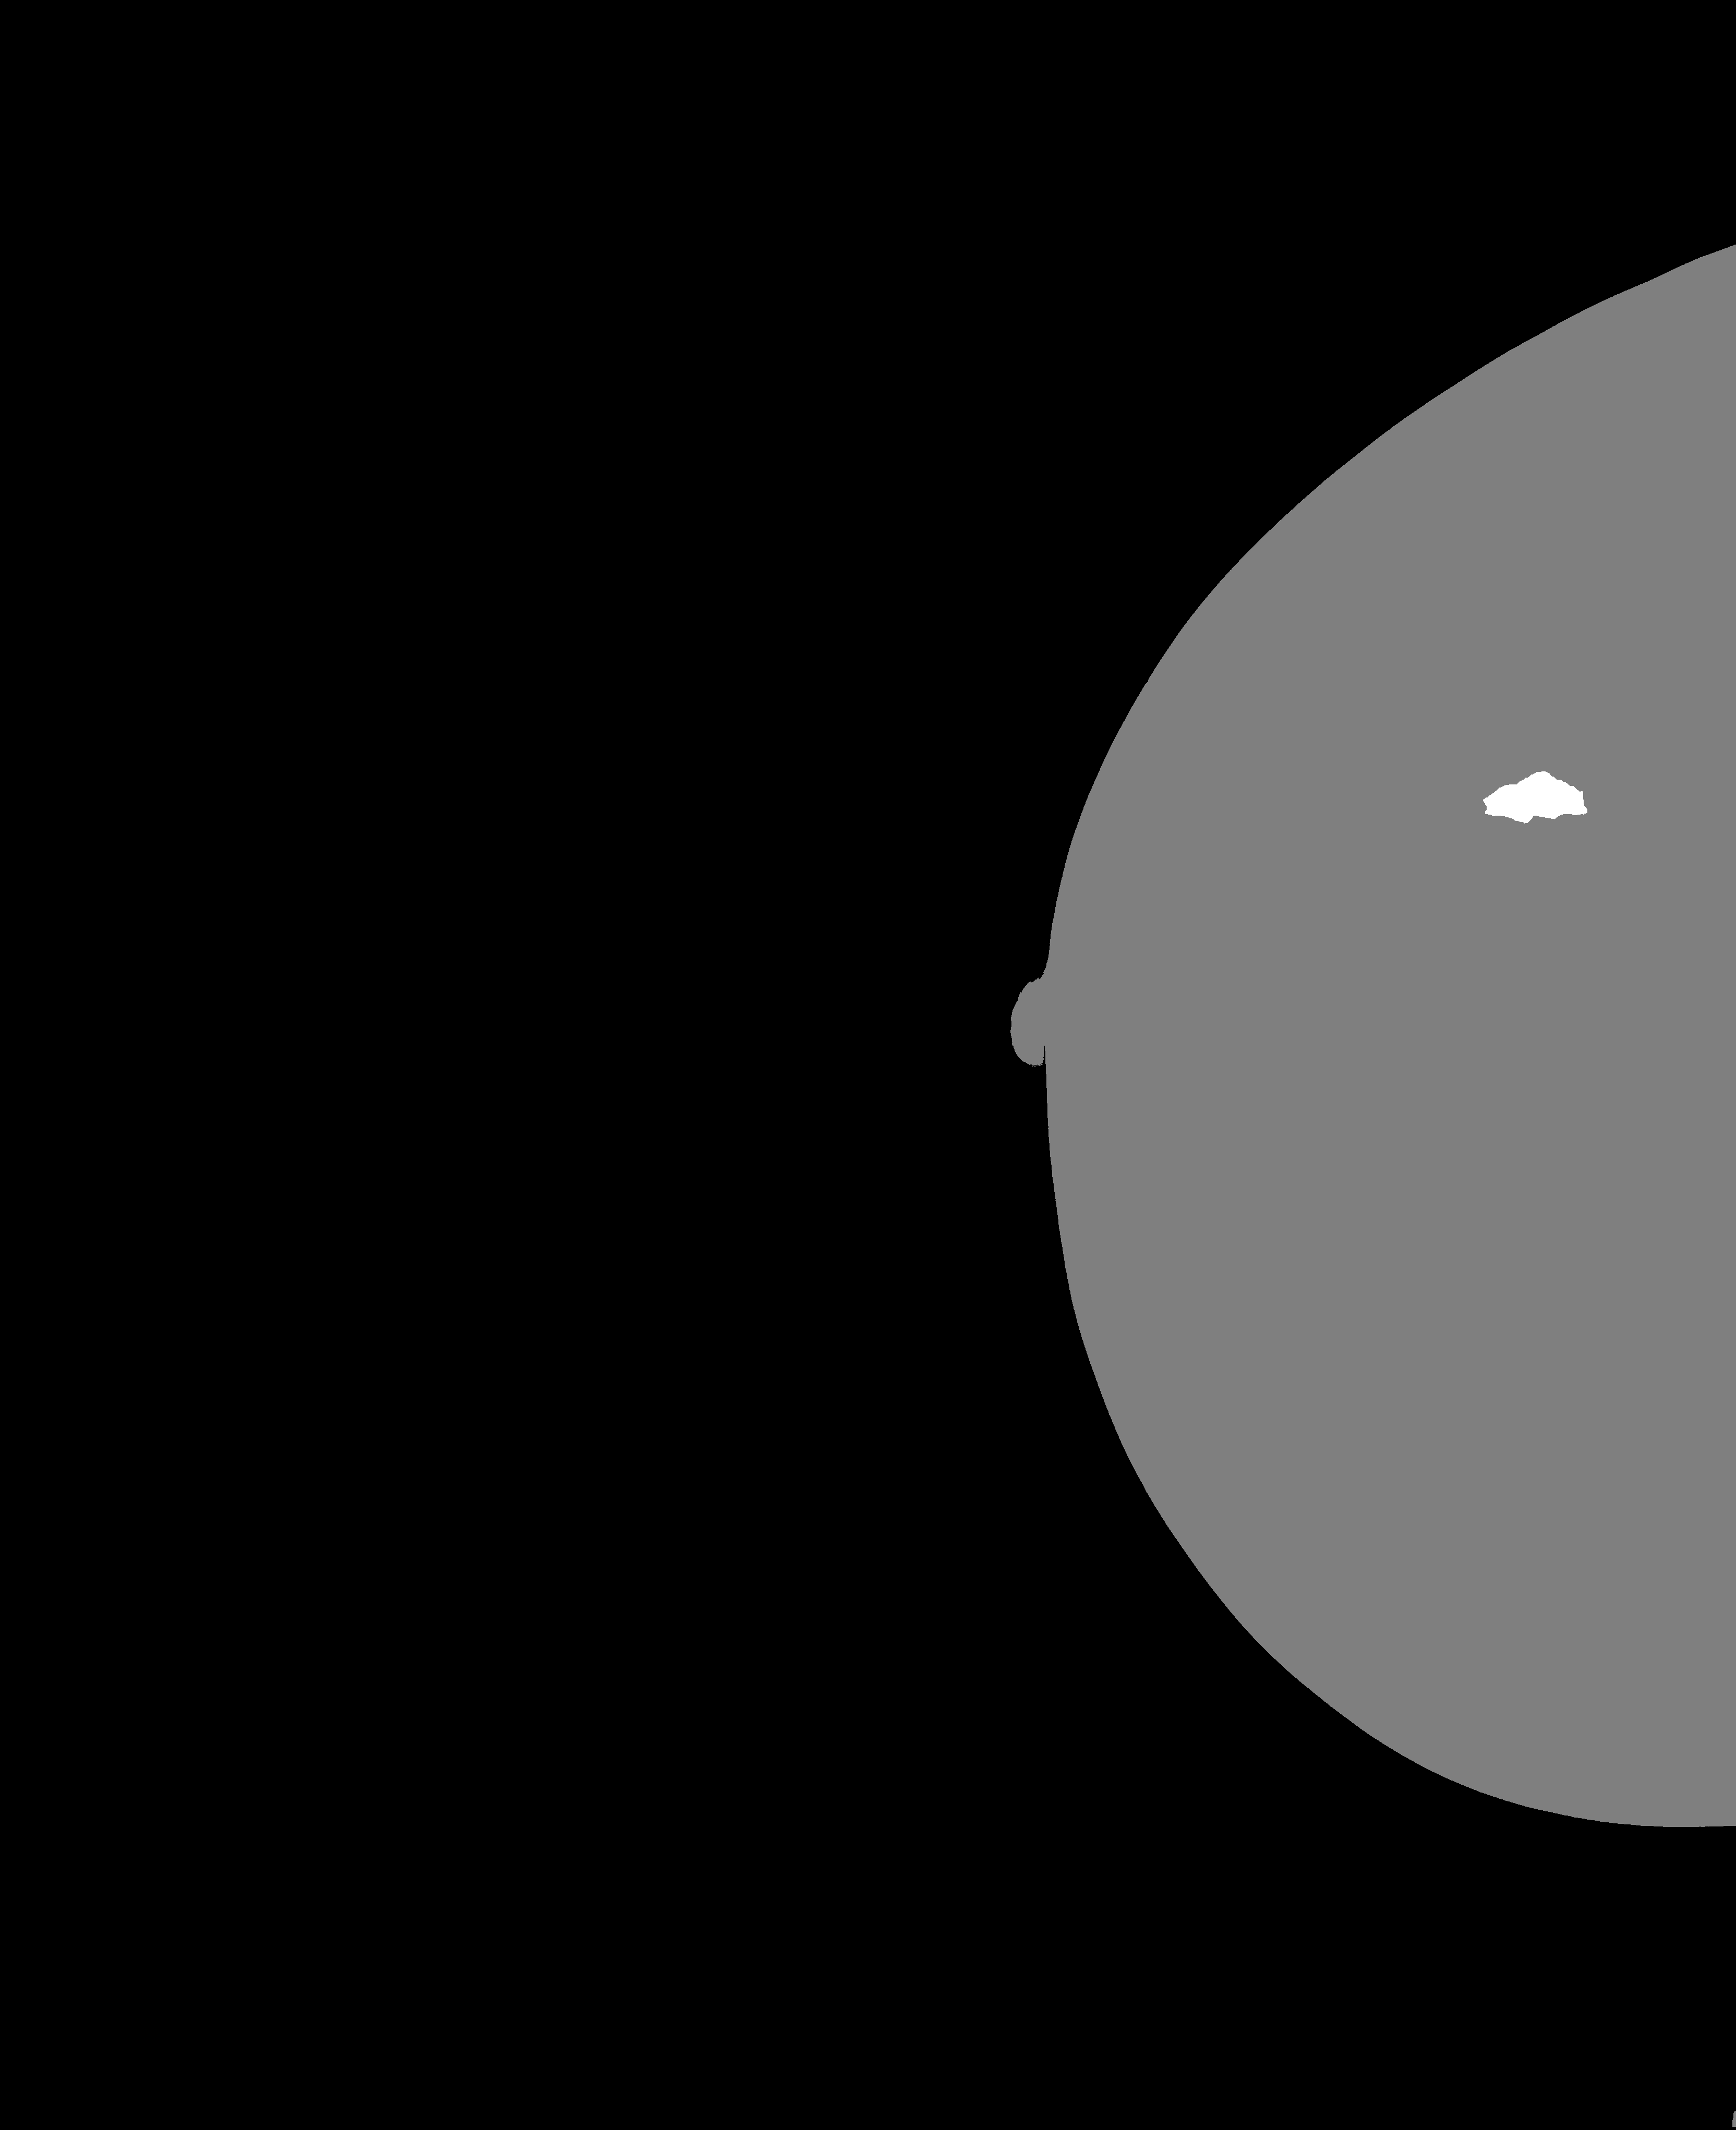
\includegraphics[width=\textwidth]{plots/label.png}
				\caption{Segmentation}
			\end{subfigure}
		% img_108_146_1_RCC.png
		\end{figure}
	\end{frame}
	
	
	\section[Convolutional networks]{Convolutional networks}
	\begin{frame}
	\frametitle{Why convolutional networks?}
		\begin{itemize}
			\item Convnets have showed great results in image classification tasks.
			\item Convnets learn which features are important for the classification. 
	 		\item We don’t need experts to carefully handcraft and select features.
		\end{itemize}
		\vfill
		Cons: Need processing power, data.
	\end{frame}
% From 2012 to now they have been used everywhere become standard in image processing, if there is a breakthrough in computer vision, most probably is donde with convnets.
% ImageNet (super-human ability) They can be used as is for image segmentation.
% Everything is learned, end-to-end

	\subsection[Classification]{Classification}
	\begin{frame}
		\frametitle{Convolutional networks}
		Learnable filters: spatially local and simple in early layers, global and complex in deeper layers.
		\begin{figure}
			\centering
			\begin{subfigure}{0.4\textwidth}
				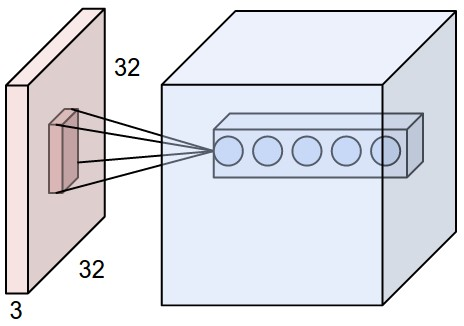
\includegraphics[width=\textwidth]{plots/convLayer.jpeg}
			\end{subfigure}
			~
			\begin{subfigure}{0.5\textwidth}
				\begin{subfigure}{\textwidth}
					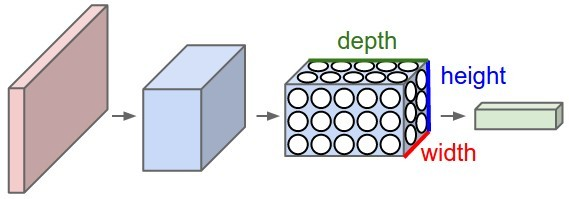
\includegraphics[width=\textwidth]{plots/convNetVolumes.jpeg}
				\end{subfigure}
				\par \smallskip
				\begin{subfigure}{\textwidth}
					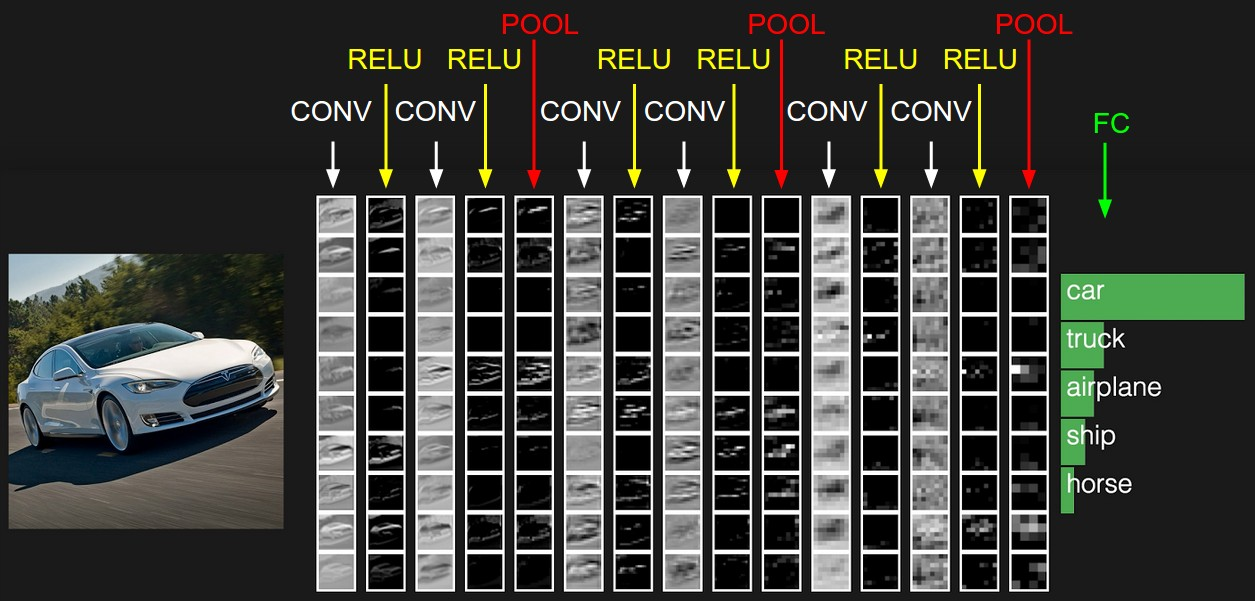
\includegraphics[width=\textwidth]{plots/convNetExample.jpeg}
				\end{subfigure}
			\end{subfigure}
		\end{figure}
		\source{[Karpathy et al., 2016]}
		
	\end{frame}
	% Explain kernels and hierarchichal features )ever more complex features).
	% hierarchical learning features and spatial invariance
	% Justificacion pooling: para que la red agregue infpormacion de diferentes lugares y vaya viendo cada vez espacios mas grandes, bigger receptive field, para aunmentar la invarianza de la ubicacion de lo que estas viendo so it recognizes it nomatter where it is and for efficiency porque redes grandes no entran en menmoria

\begin{comment}		
	\begin{frame}
		\frametitle{Object classification}
		\vspace{30pt}
		\begin{figure}
			\centering
			\begin{subfigure}{\textwidth}
				
\includegraphics[width=\textwidth]{plots/imageNetLogo.png}
			\end{subfigure}
			\par\smallskip
			\begin{subfigure}{0.35\textwidth}
				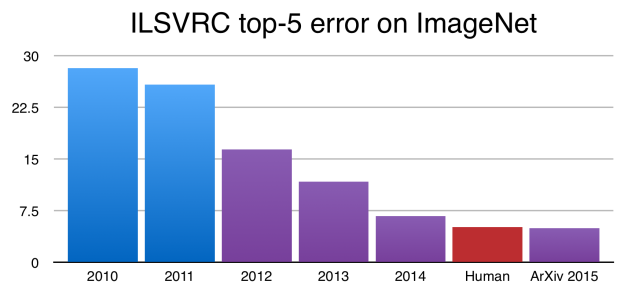
\includegraphics[width=\textwidth]{plots/imageNetAdvances.png}
			\end{subfigure}
			~
			\begin{subfigure}{0.6\textwidth}
				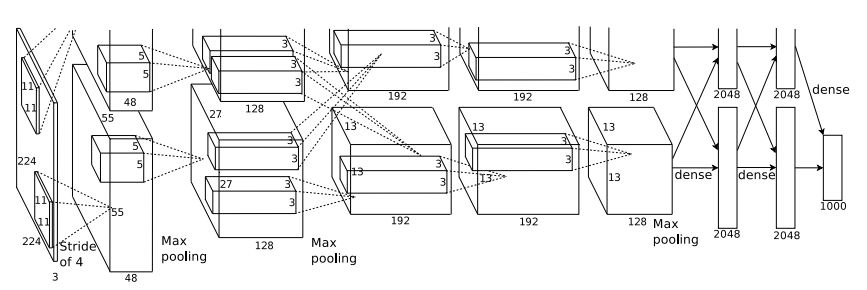
\includegraphics[width=\textwidth]{plots/alexnet.png}
			\end{subfigure}
		\end{figure}
		\source{[Nvidia Corp., 2015], [Krizhevsky et al., 2012]}
		% Explain ImageNet and talk about results
	\end{frame}
	
	\begin{frame}
		\frametitle{Architectures}
		\begin{figure}
			\centering
			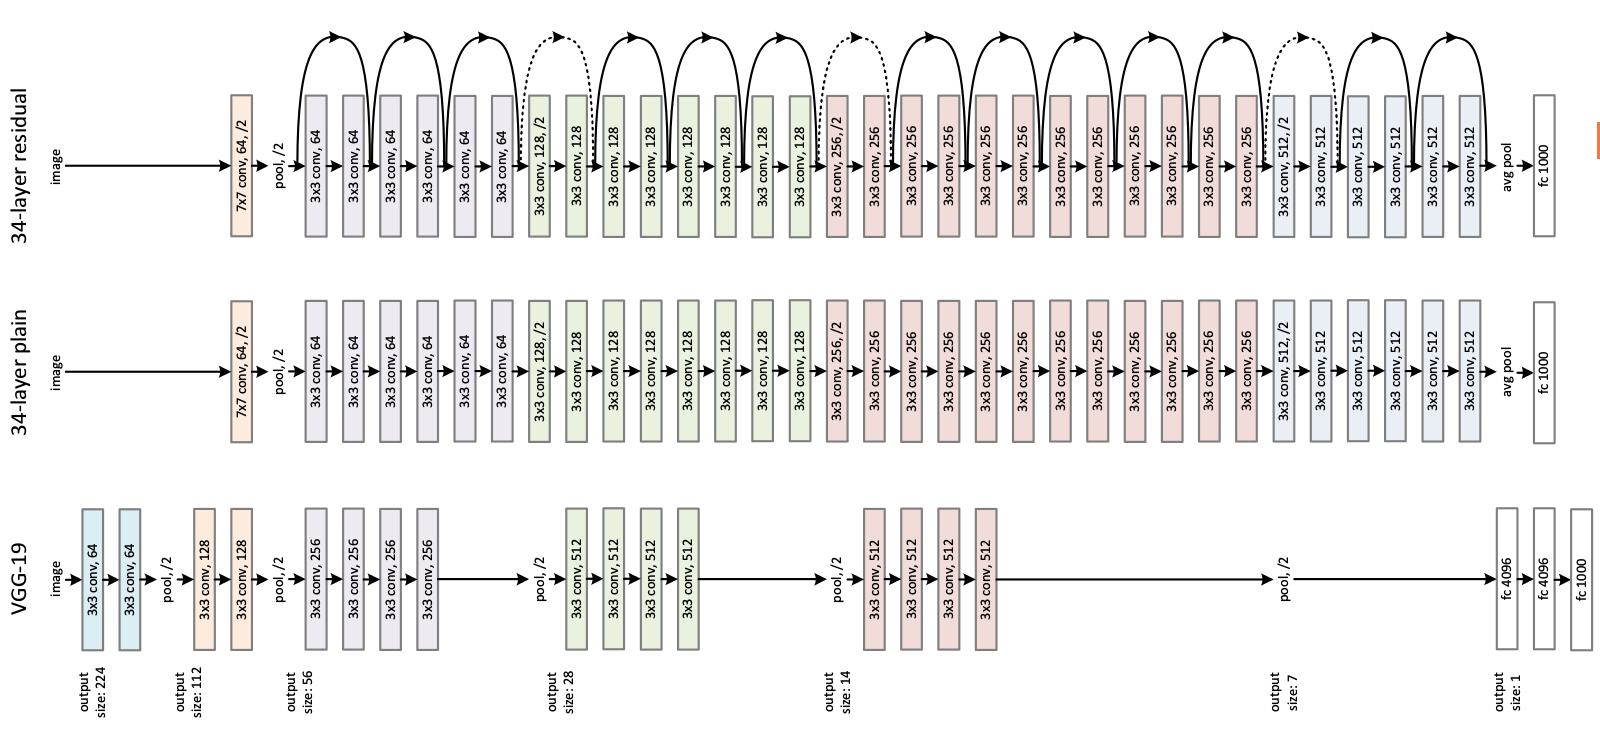
\includegraphics[width=\textwidth]{plots/resNet.png}
		\end{figure}
		
		Deeper, no pooling layers, no fully-connected layers, no dropout, all 3x3 kernels, batch normalization, residual connections, attention, memory...
		\source{[He et al., 2015]}
		% VGG-net and ResNet-like/other things
		% Deeper, no pooling, no fc, no dropout, batchnorm, residual connections
		% all 3x3 convolutions
	\end{frame}
\end{comment}
	\subsection[Segmentation]{Segmentation}
	\begin{frame}
		\frametitle{Segmentation}
		Solved by upsampling, deconvolution or dilated convolutions.
		\begin{figure}
			\centering
			\begin{subfigure}{0.47\textwidth}
				\begin{subfigure}{\textwidth}
					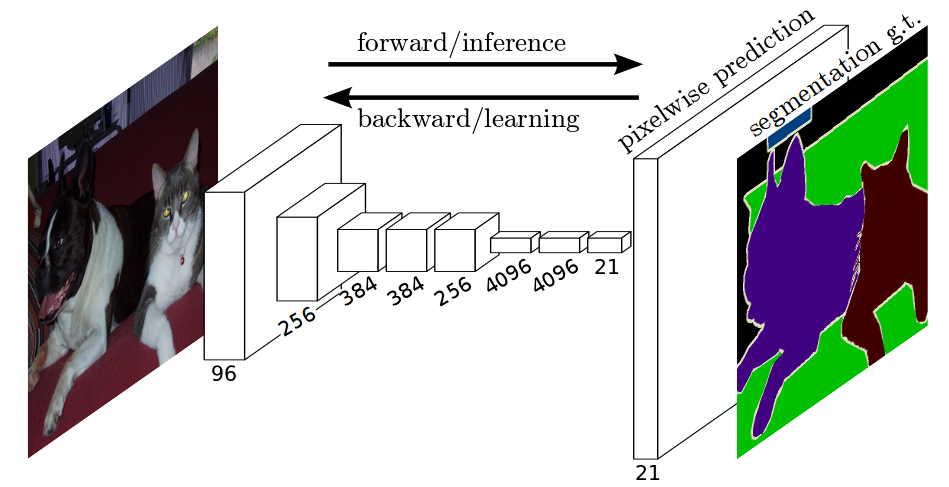
\includegraphics[width=\textwidth]{plots/fcn.png}
				\end{subfigure}
				\par \bigskip
				\begin{subfigure}{\textwidth}
					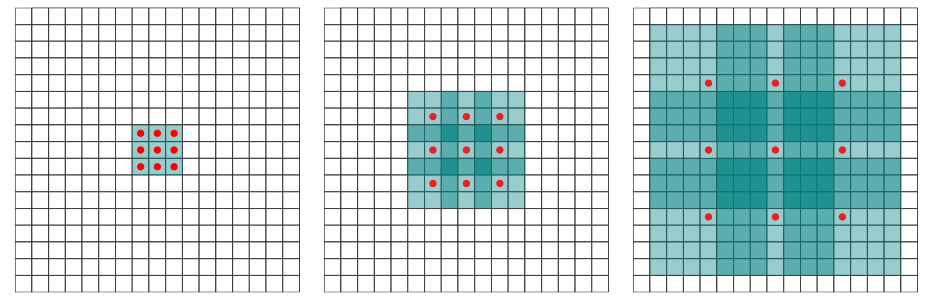
\includegraphics[width=\textwidth]{plots/dilated.png}
				\end{subfigure}
			\end{subfigure}
			~
			\begin{subfigure}{0.5\textwidth}
				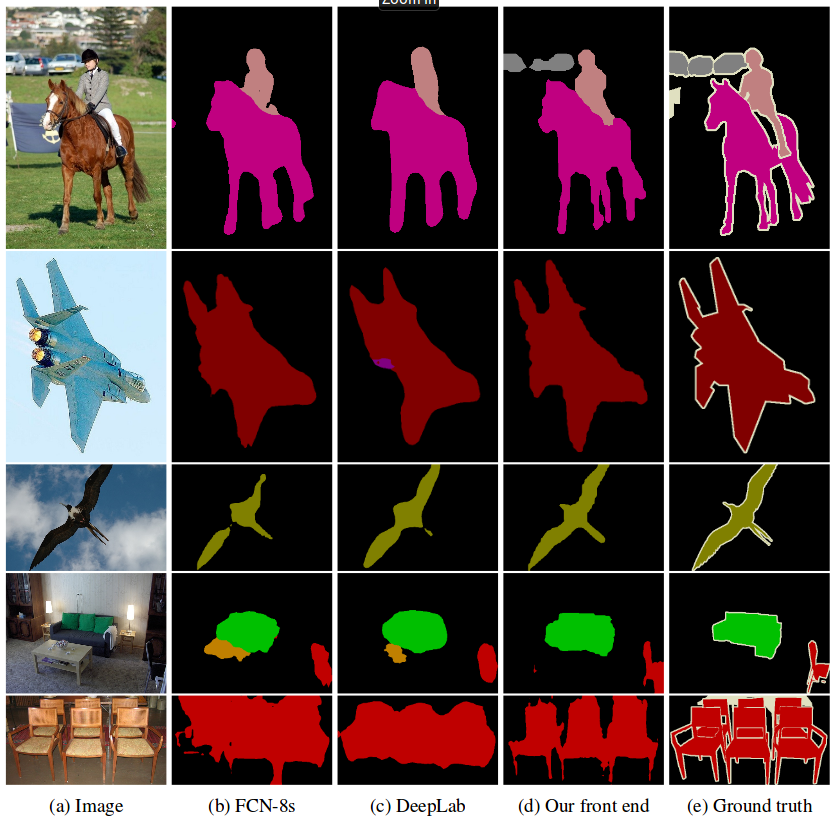
\includegraphics[width=\textwidth]{plots/segmentationComparison.png}
			\end{subfigure}
		\end{figure}
		\source{[Long et al., 2015], [Yu and Koltun, 2016]}
		% Explain how kernels are moved along to produce a full result
	\end{frame}
	% Traditional way. Image visión, specialized techniques. Handcrafted features made by experts But it is hard to design this, and it takes time to maintain, and you need expertise: end-to-end, learn from data, not done by hand. Pipeline
	% Completely automatic, single step v. pipeline.
	\begin{frame}
	    \frametitle{Example}
	    Selected feature maps from different layers.
	    
	    \begin{figure}
	        \begin{subfigure}{0.19\textwidth}
		        \centering
			        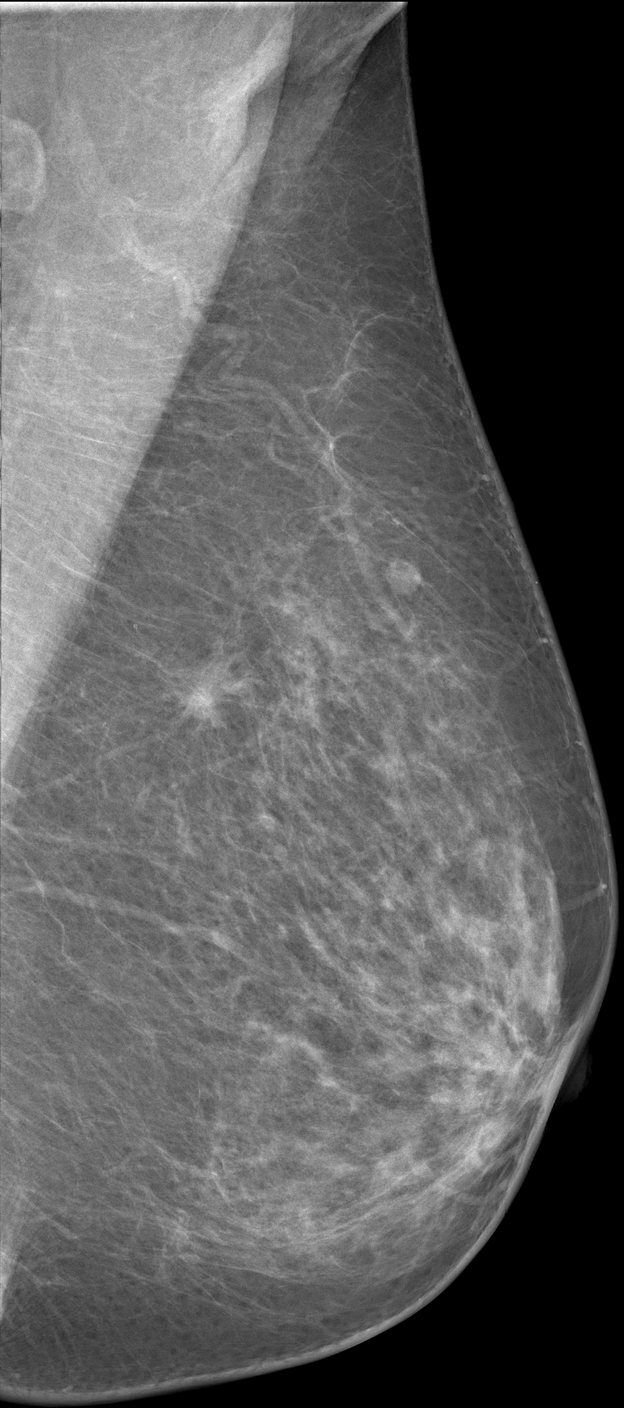
\includegraphics[width=\textwidth]{plots/layer_0.png}
		        \caption{Input ($1408 \times 624$)}
            \end{subfigure}
	        \begin{subfigure}{0.19\textwidth}
		        \centering
			        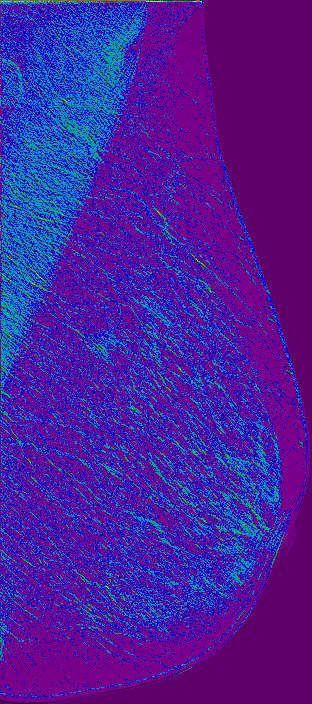
\includegraphics[width=\textwidth]{plots/layer_1.png}
		        \caption{Layer 1 ($704 \times 312$)}
            \end{subfigure}
	        \begin{subfigure}{0.19\textwidth}
		        \centering
			        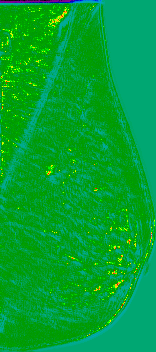
\includegraphics[width=\textwidth]{plots/layer_4.png}
		        \caption{Layer 4 ($352 \times 156$)}
            \end{subfigure}
	        \begin{subfigure}{0.19\textwidth}
		        \centering
			        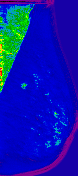
\includegraphics[width=\textwidth]{plots/layer_7.png}
		        \caption{Layer 7 ($176 \times 78$)}
            \end{subfigure}
            \begin{subfigure}{0.19\textwidth}
		        \centering
			        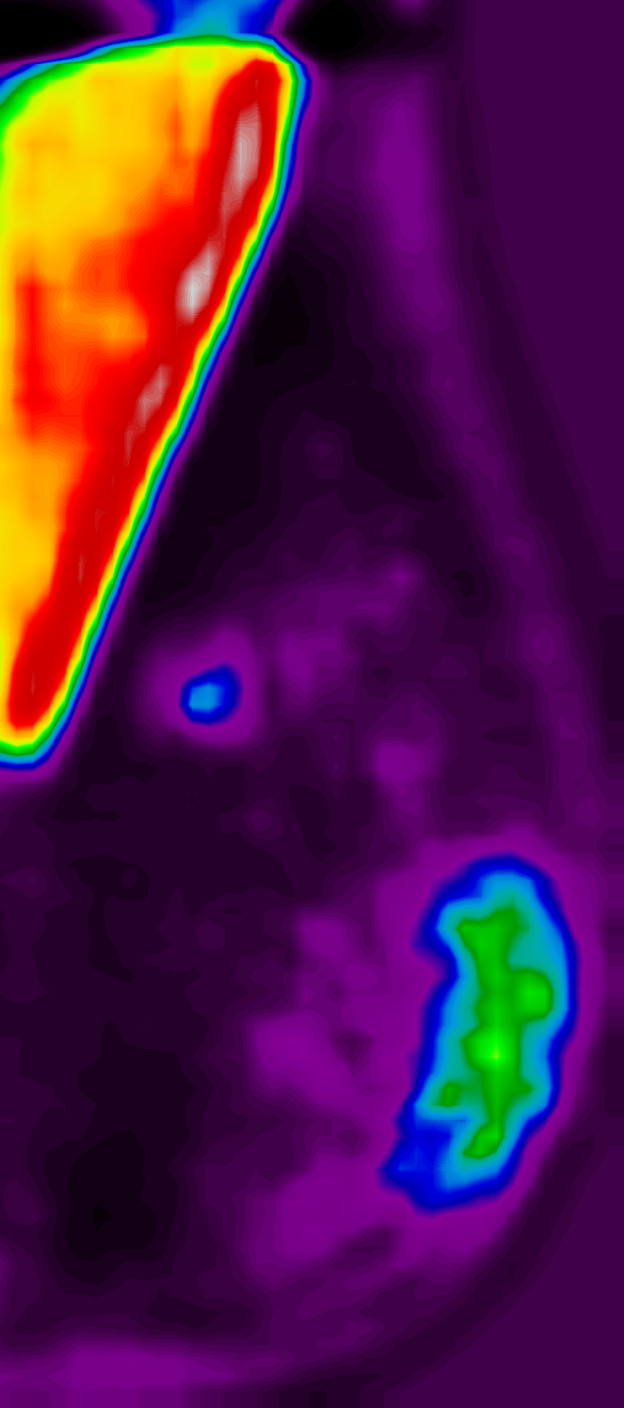
\includegraphics[width=\textwidth]{plots/layer_9.png}
		        \caption{Output ($1408 \times 624$)}
            \end{subfigure}
        \end{figure}
	\end{frame}


	\section[Experiments]{Experiments}
	\begin{frame}
		\frametitle{Literature review}
		\vspace{15pt}
		\begin{figure}
			\centering
			\begin{subfigure}{0.48\textwidth}
				\begin{subfigure}{\textwidth}
					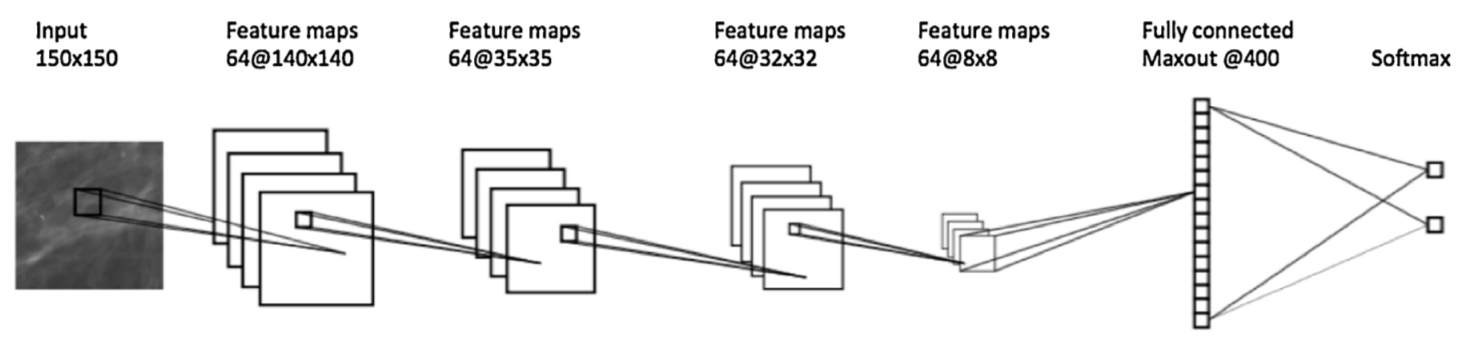
\includegraphics[width=\textwidth]{plots/arevalo.png}
				\end{subfigure}
				~
				\begin{subfigure}{\textwidth}
					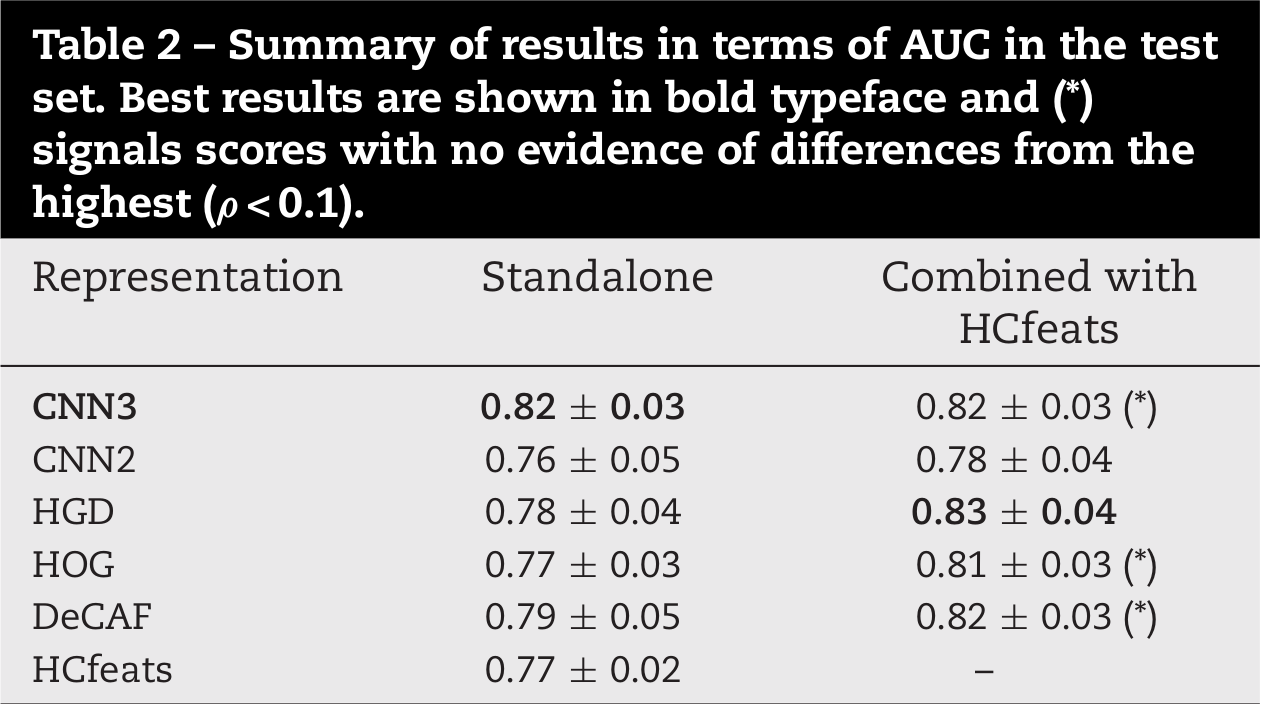
\includegraphics[width=\textwidth]{plots/arevaloResults.png}
				\end{subfigure}
				\caption{Mass diagnosis (4 layers, 3.4M params)}
			\end{subfigure}
			~
			\begin{subfigure}{0.48\textwidth}
				\begin{subfigure}{\textwidth}
					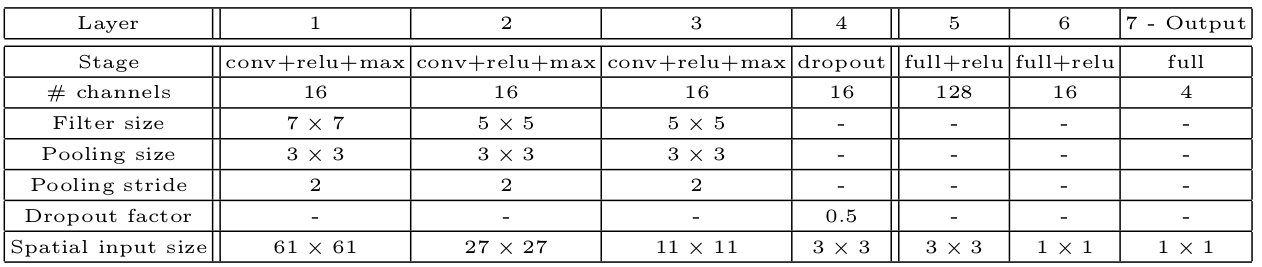
\includegraphics[width=\textwidth]{plots/dubrovina1.png}
				\end{subfigure}
				~
				\begin{subfigure}{\textwidth}
					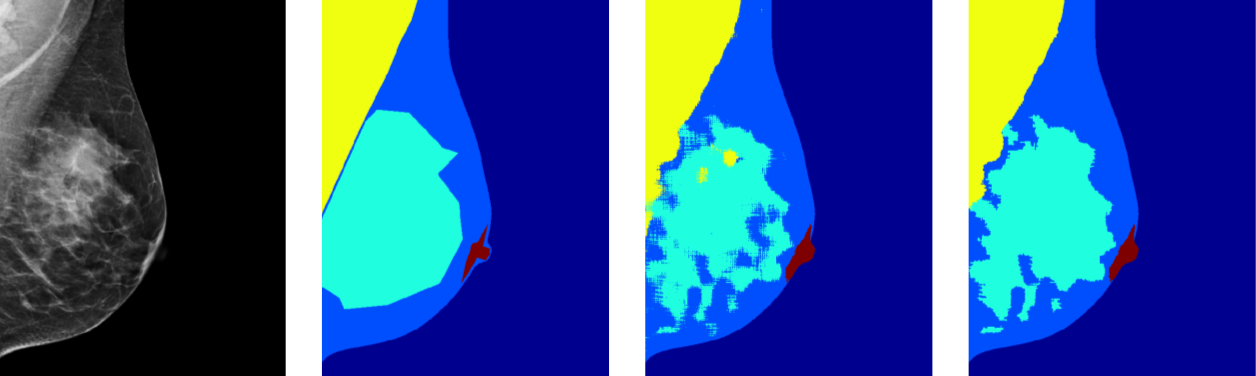
\includegraphics[width=\textwidth]{plots/dubrovina2.png}
				\end{subfigure}
				~
				\begin{subfigure}{\textwidth}
					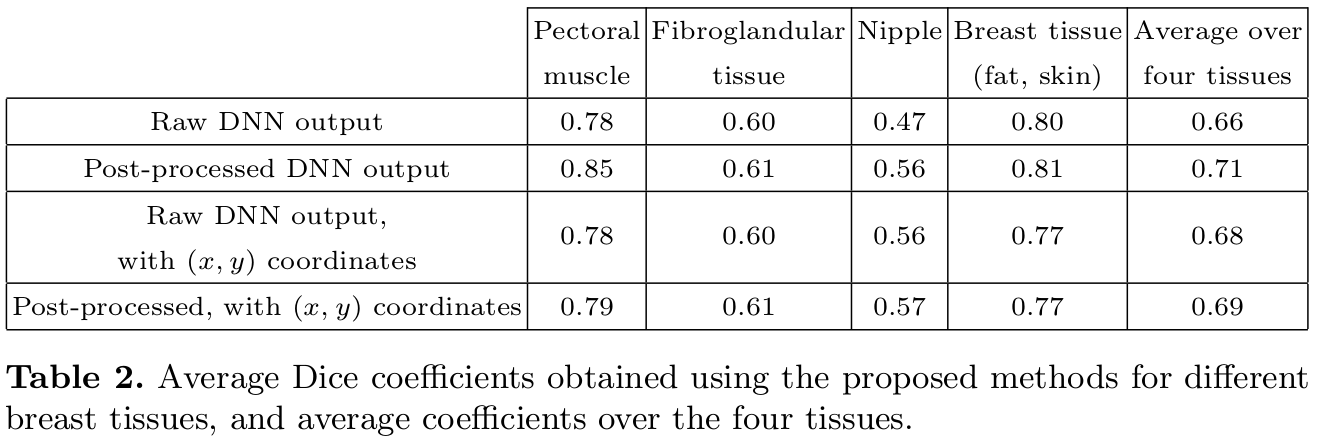
\includegraphics[width=\textwidth]{plots/dubrovinaResults.png}
				\end{subfigure}
				\caption{Tissue segmentation (6 layers, 34K params)}
			\end{subfigure}
		\end{figure}
		\source{[Arevalo et al., 2016], [Dubrovina et al.,2015]}
		% What has been done in breast cancer, Wrote background, examples and accuracies
	\end{frame}
	
    \begin{frame}
        \frametitle{Database}
        Our mammographic database provided by the Breast Cancer Digital Repository Consortium consists of 256 digital mammograms from 63 Portuguese patients with at least one breast mass. % 139 in total
        
        We augment the data set for training.
        \small
        \begin{table}[h]
	        \centering
	        \begin{tabular}{lcccccccc}
		        \hline
		        & \multicolumn{2}{c}{\textbf{Patients}} & \multicolumn{2}{c}{\textbf{Mammograms}} &\multicolumn{2}{c}{\textbf{Masses}}\\
		        & \textbf{Training} & \textbf{Test} & \textbf{Training} & \textbf{Test} & \textbf{Training} & \textbf{Test} \\
		        \hline 
		        Fold 1	&50	&13	&189	&67	&106	&33\\
		        Fold 2	&50	&13	&209	&47	&112	&27\\
		        Fold 3	&50	&13	&204	&52	&110	&29\\
		        Fold 4	&51	&12	&209	&47	&110	&29\\
		        Fold 5	&51	&12 &213	&43	&118	&21\\
		        Average &50.6 &12.6 &204.8 &51.2 &111.2 &27.8\\
		        \hline
	        \end{tabular}
        \end{table}
        \source[Moura et al., 2013]
    \end{frame}
    
	\begin{frame}
		\frametitle{Preprocessing}
		\begin{figure}
		\centering
			\begin{subfigure}{0.24\textwidth}
				\centering
					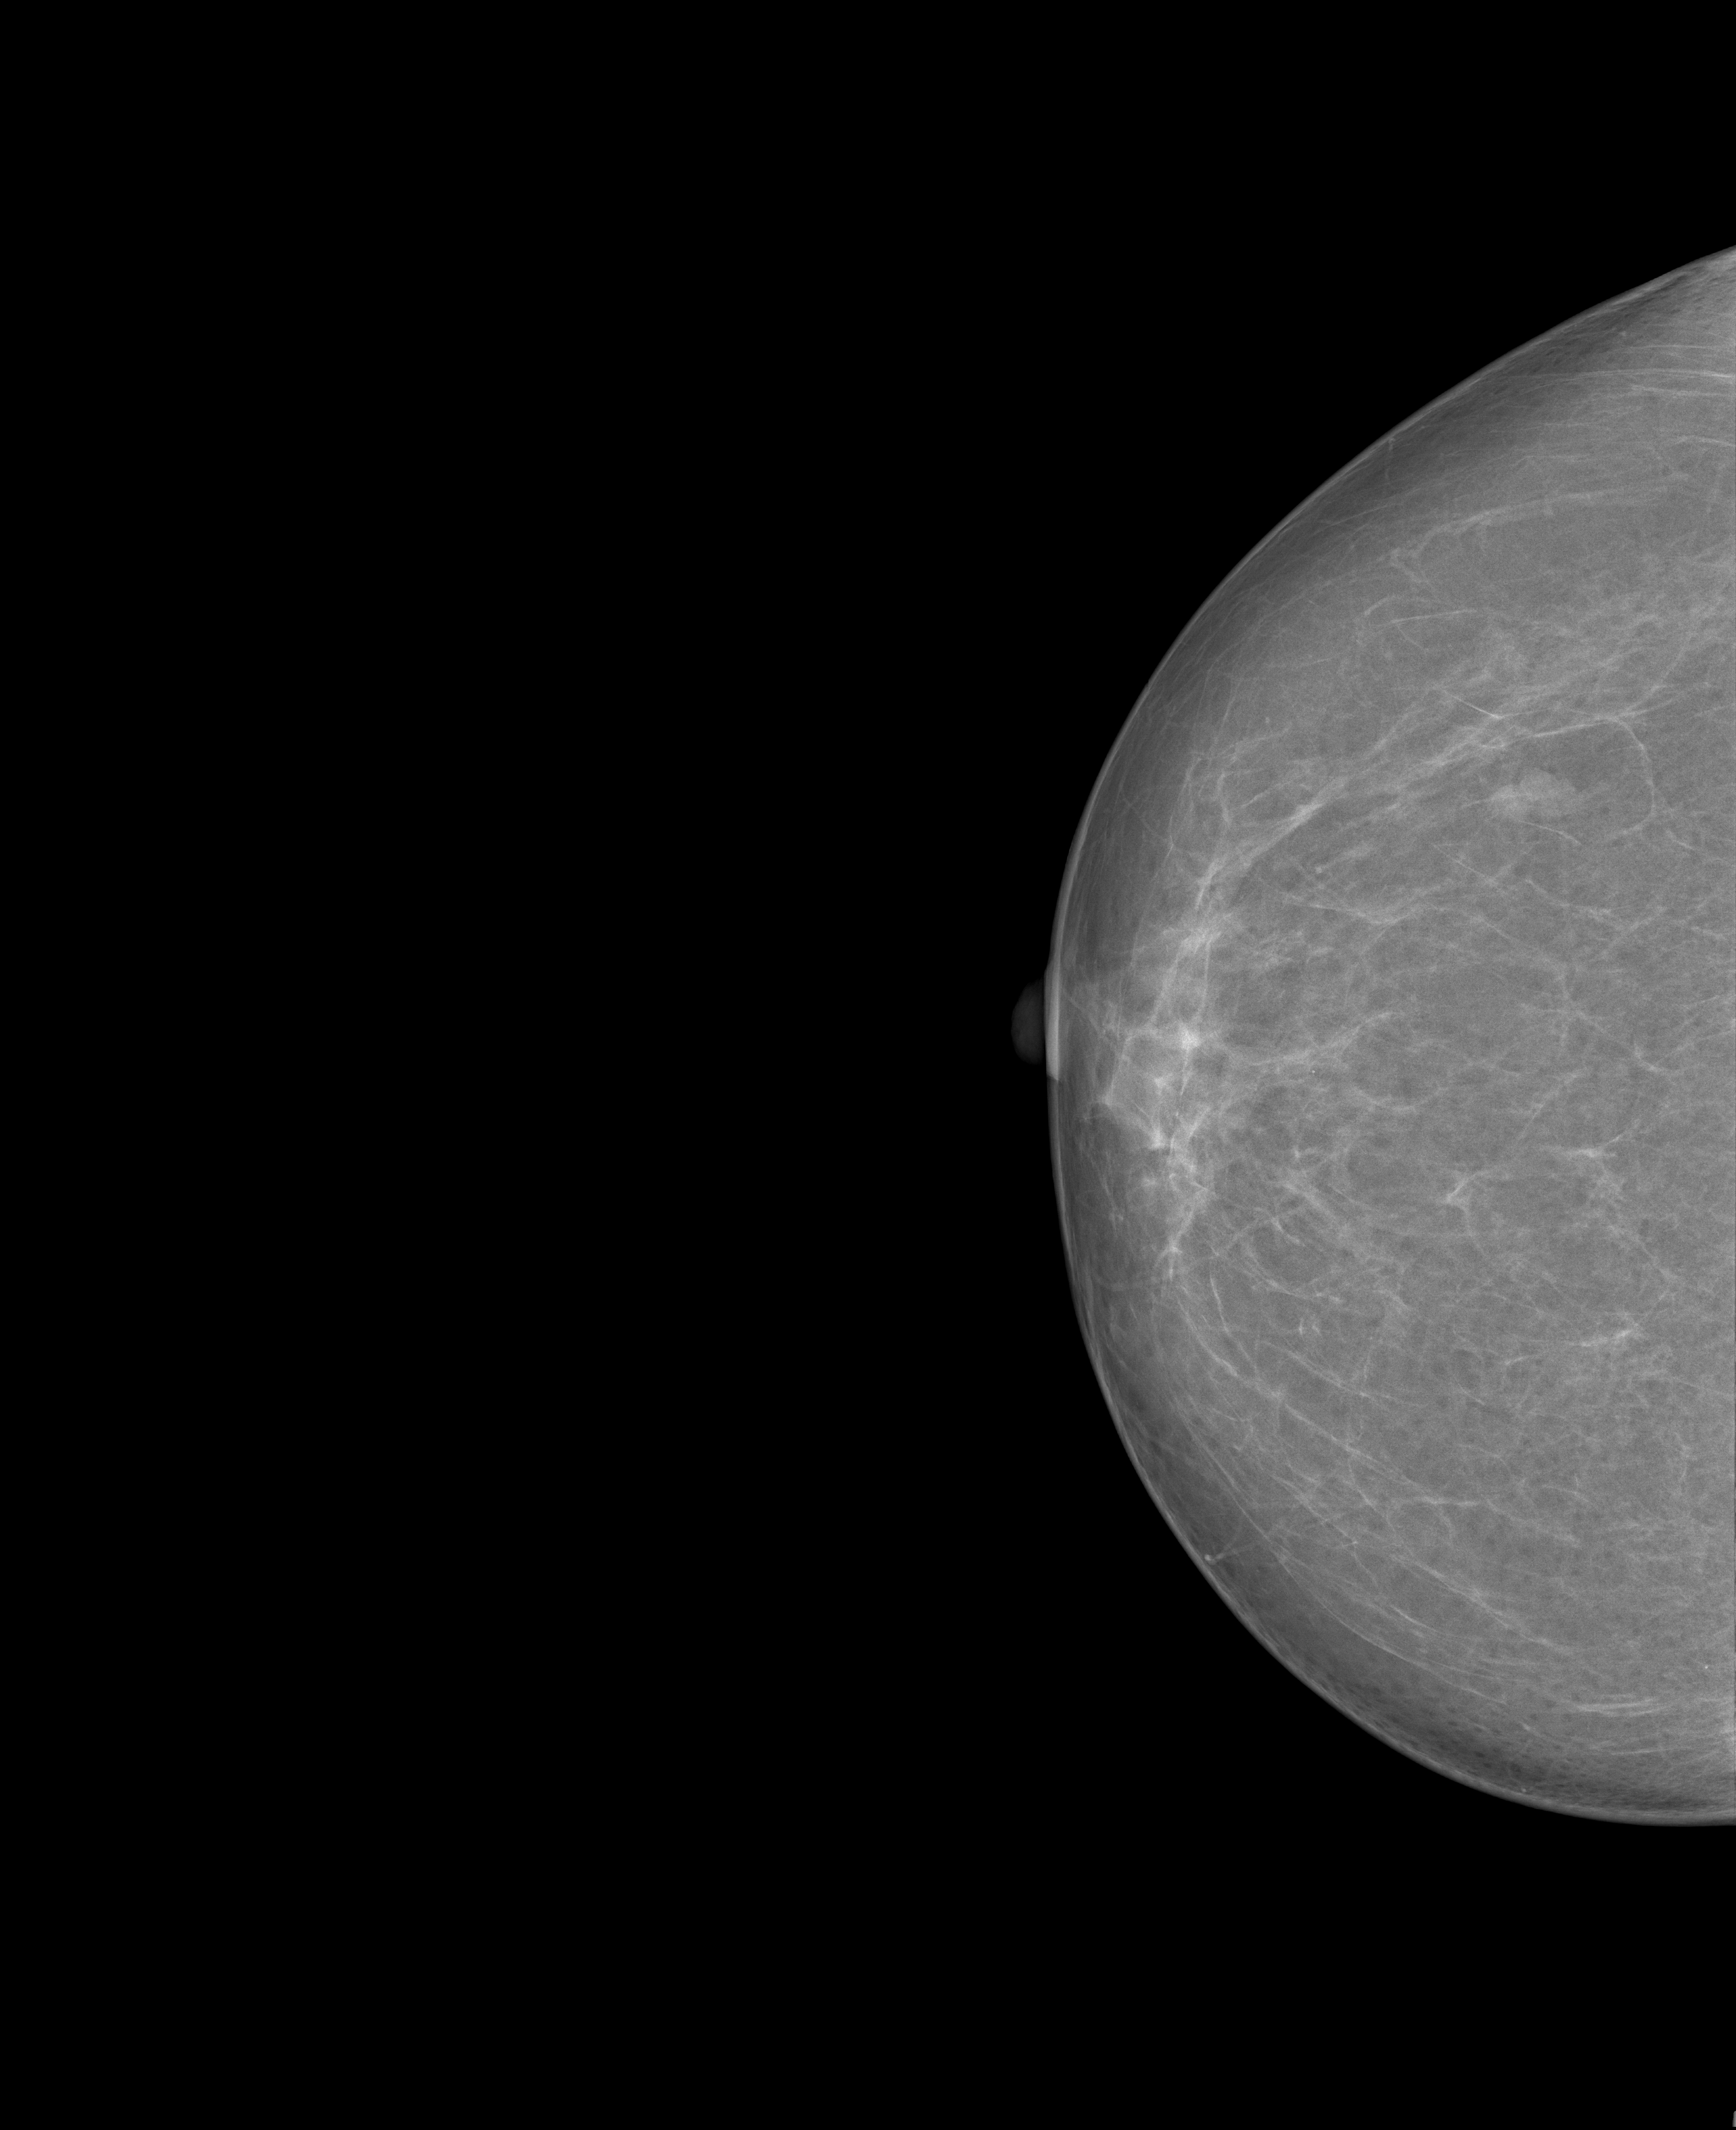
\includegraphics[height=3.5cm]{plots/mammogram.png}
			\end{subfigure}
			\begin{subfigure}{0.24\textwidth}
				\centering
					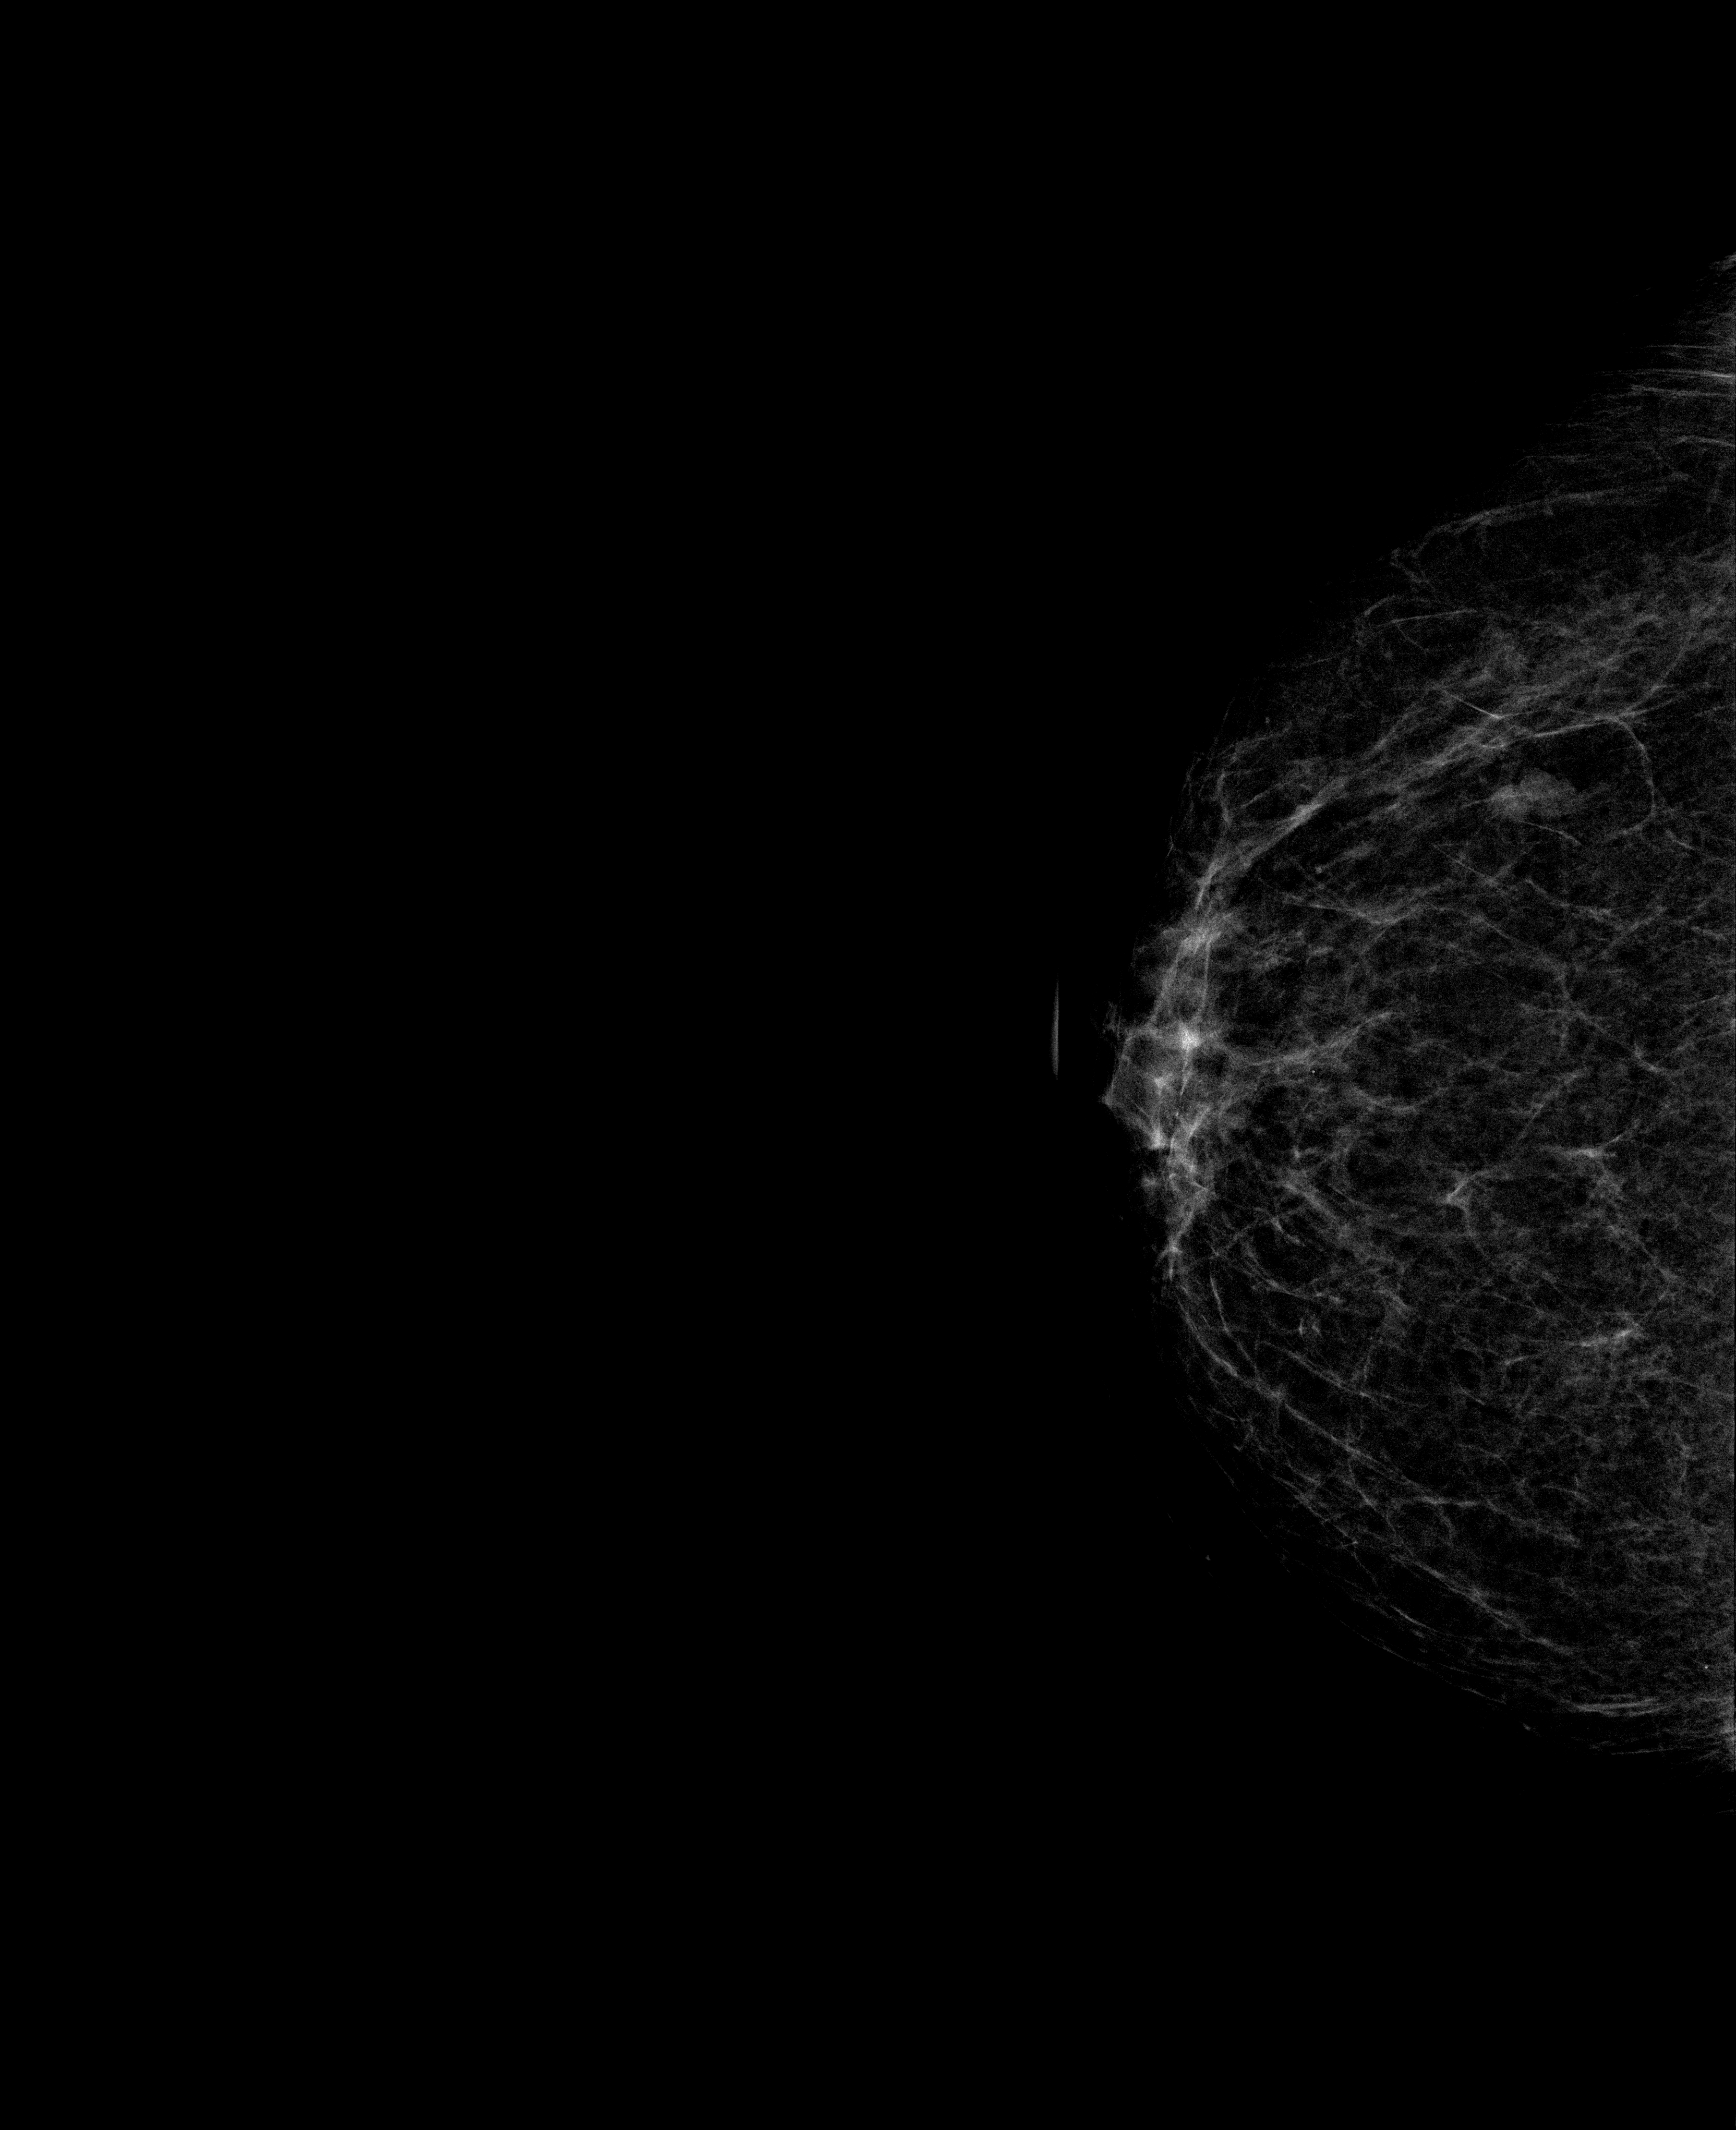
\includegraphics[height=3.5cm]{plots/mammogram_enhanced.png}
			\end{subfigure}
			\begin{subfigure}{0.24\textwidth}
				\centering
					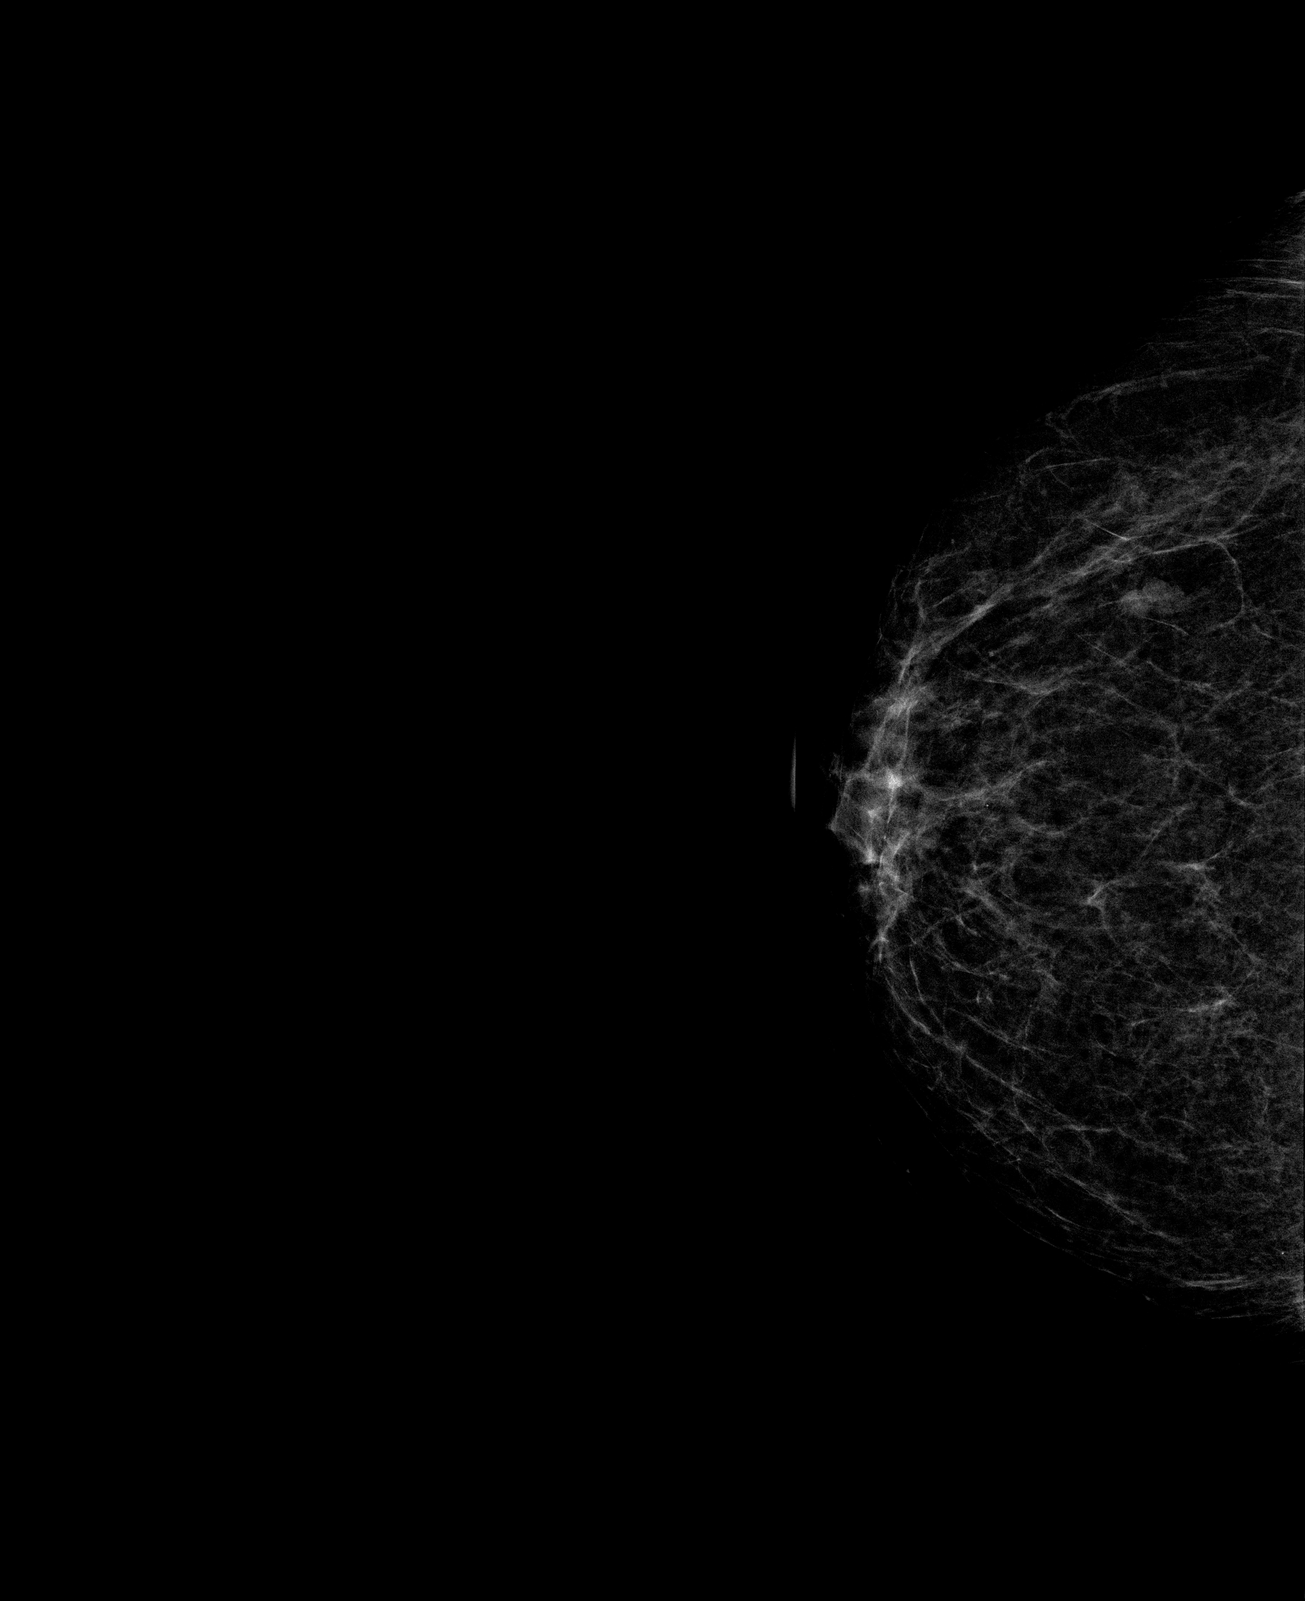
\includegraphics[height=3.5cm]{plots/mammogram_resized.png}
			\end{subfigure}
			\begin{subfigure}{0.11\textwidth}
				\centering
					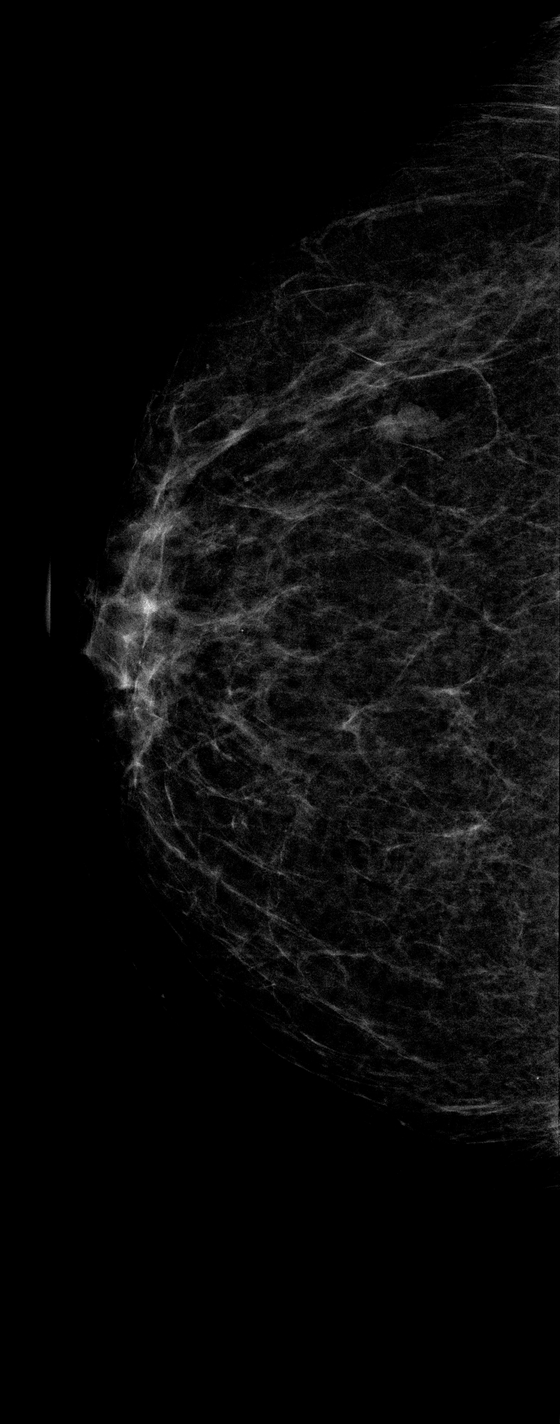
\includegraphics[height=3.5cm]{plots/mammogram_final.png}
			\end{subfigure}
			~
			\begin{subfigure}{0.24\textwidth}
				\centering
					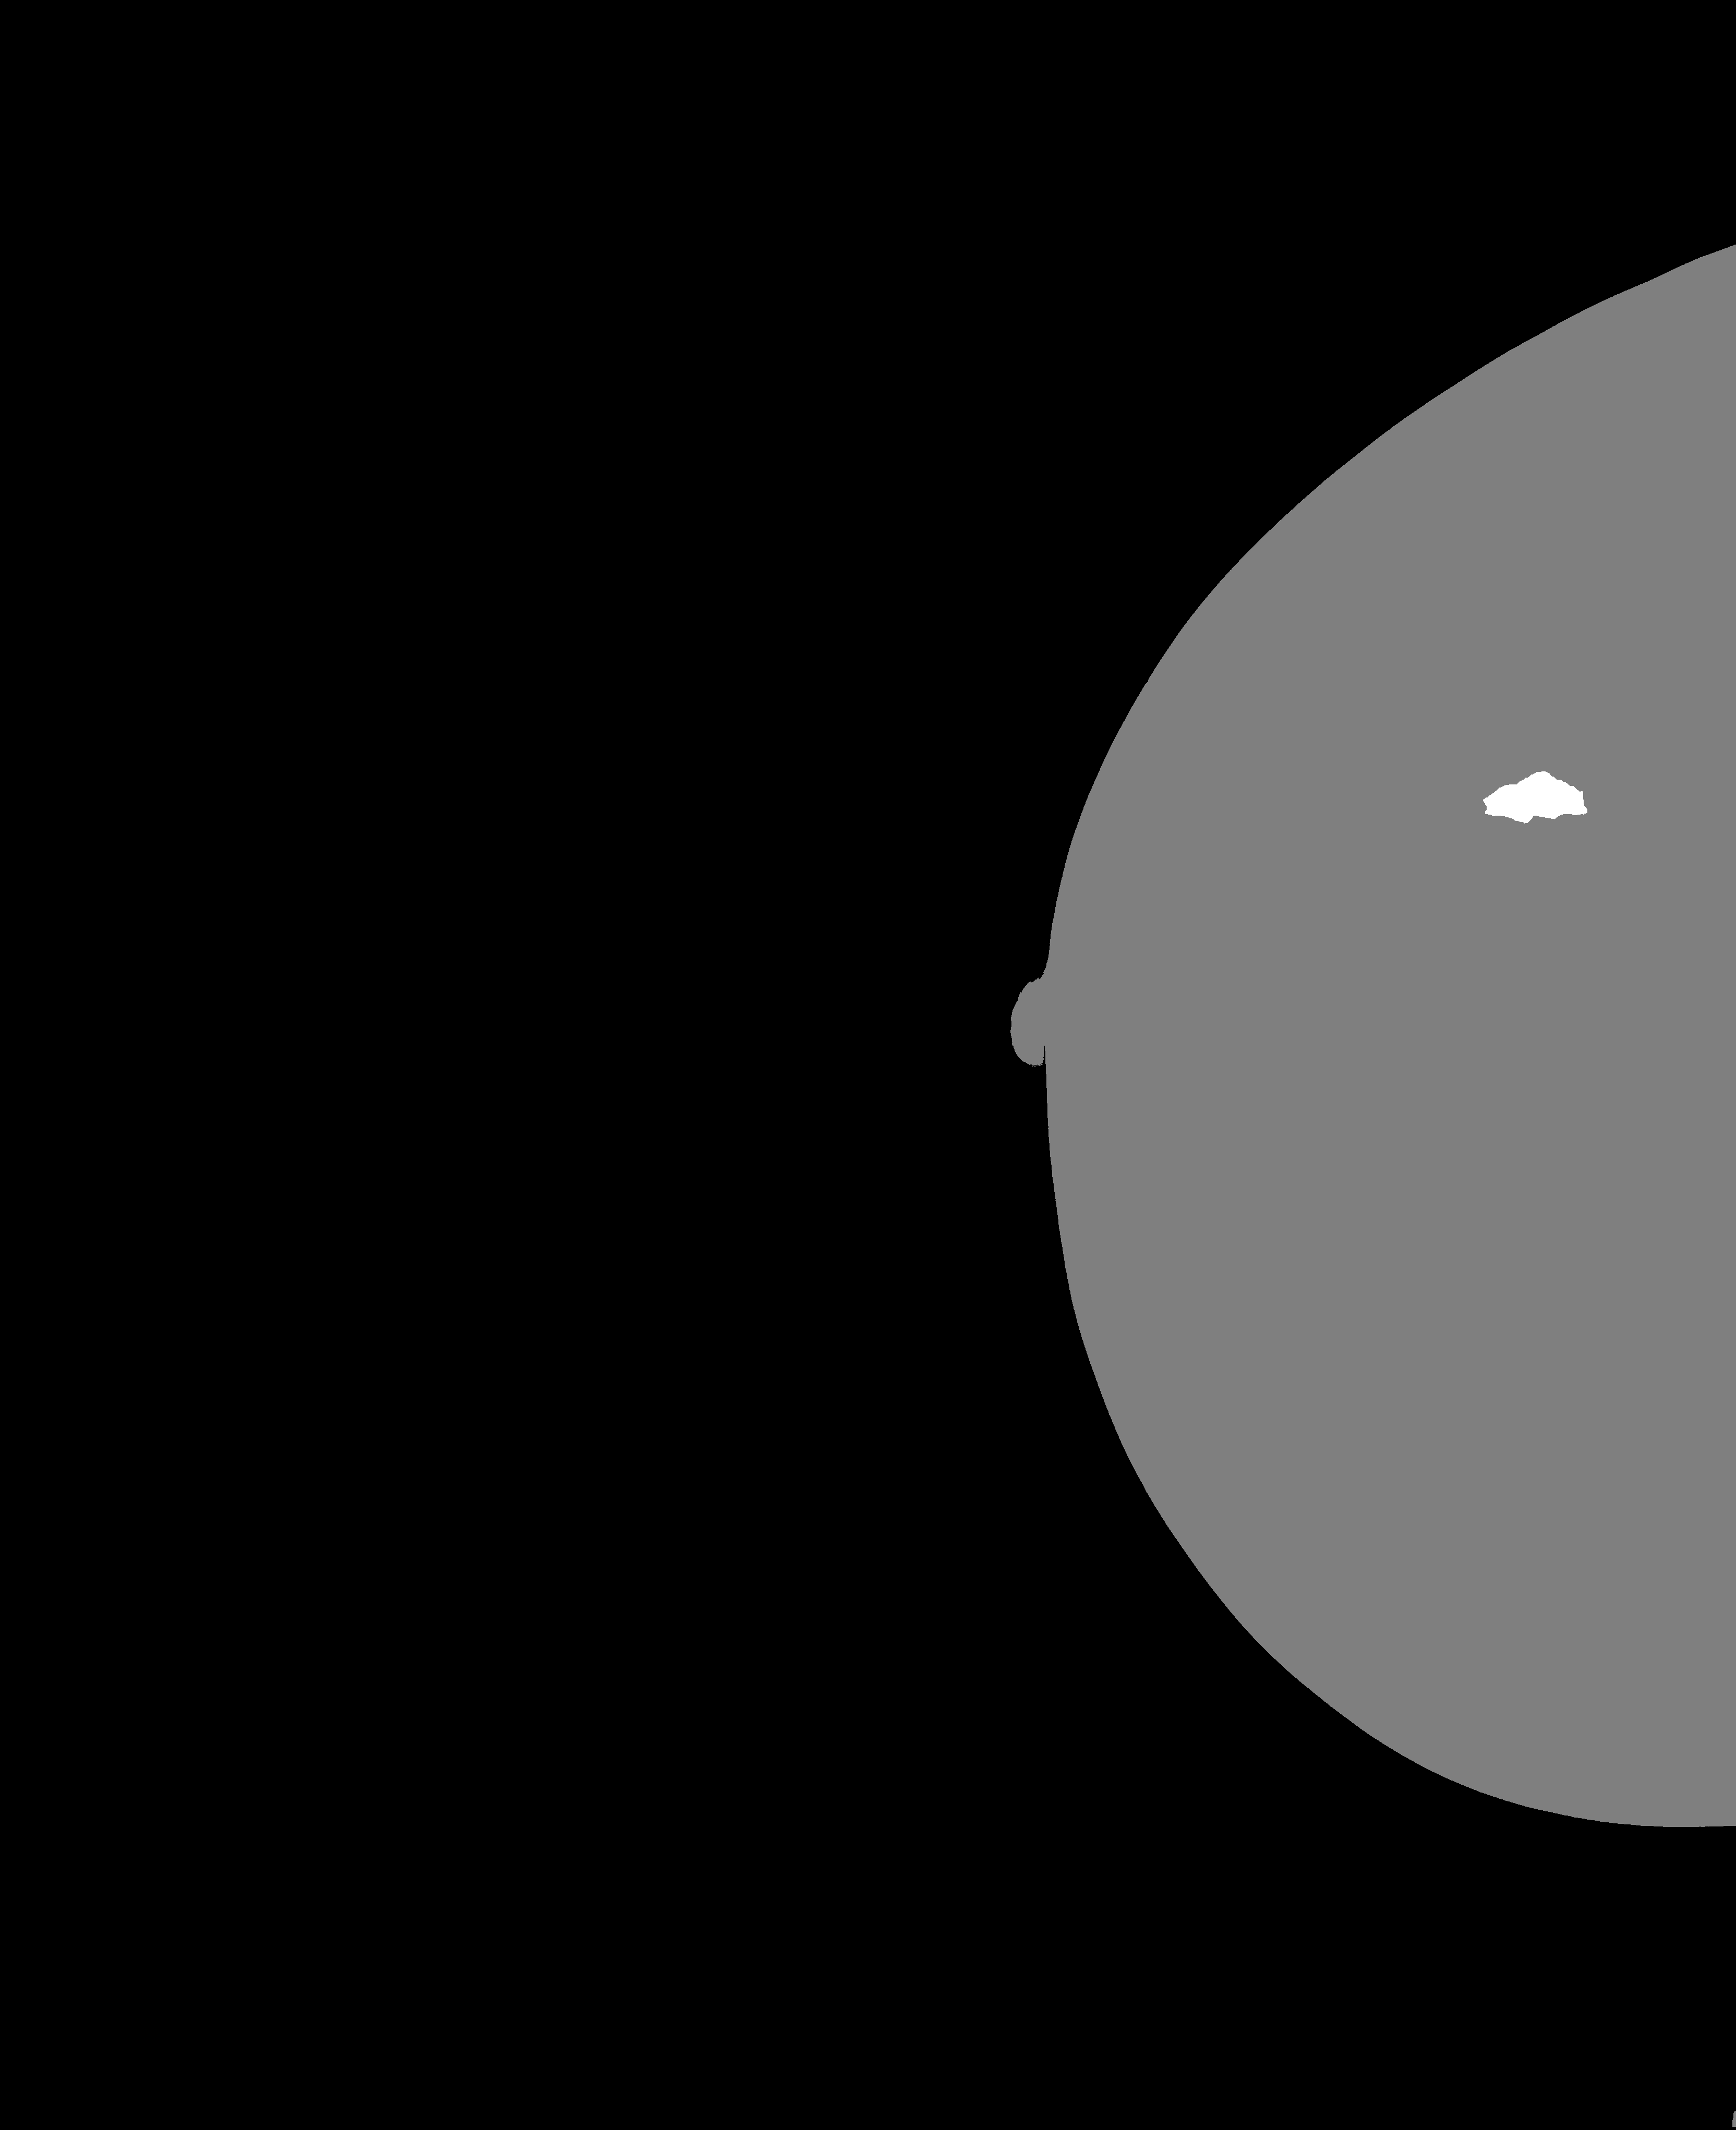
\includegraphics[height = 3.5cm]{plots/label.png}
				\caption{Original image}
				\label{subfig:Preprocessinga}
			\end{subfigure}
			\begin{subfigure}{0.24\textwidth}
				\centering
					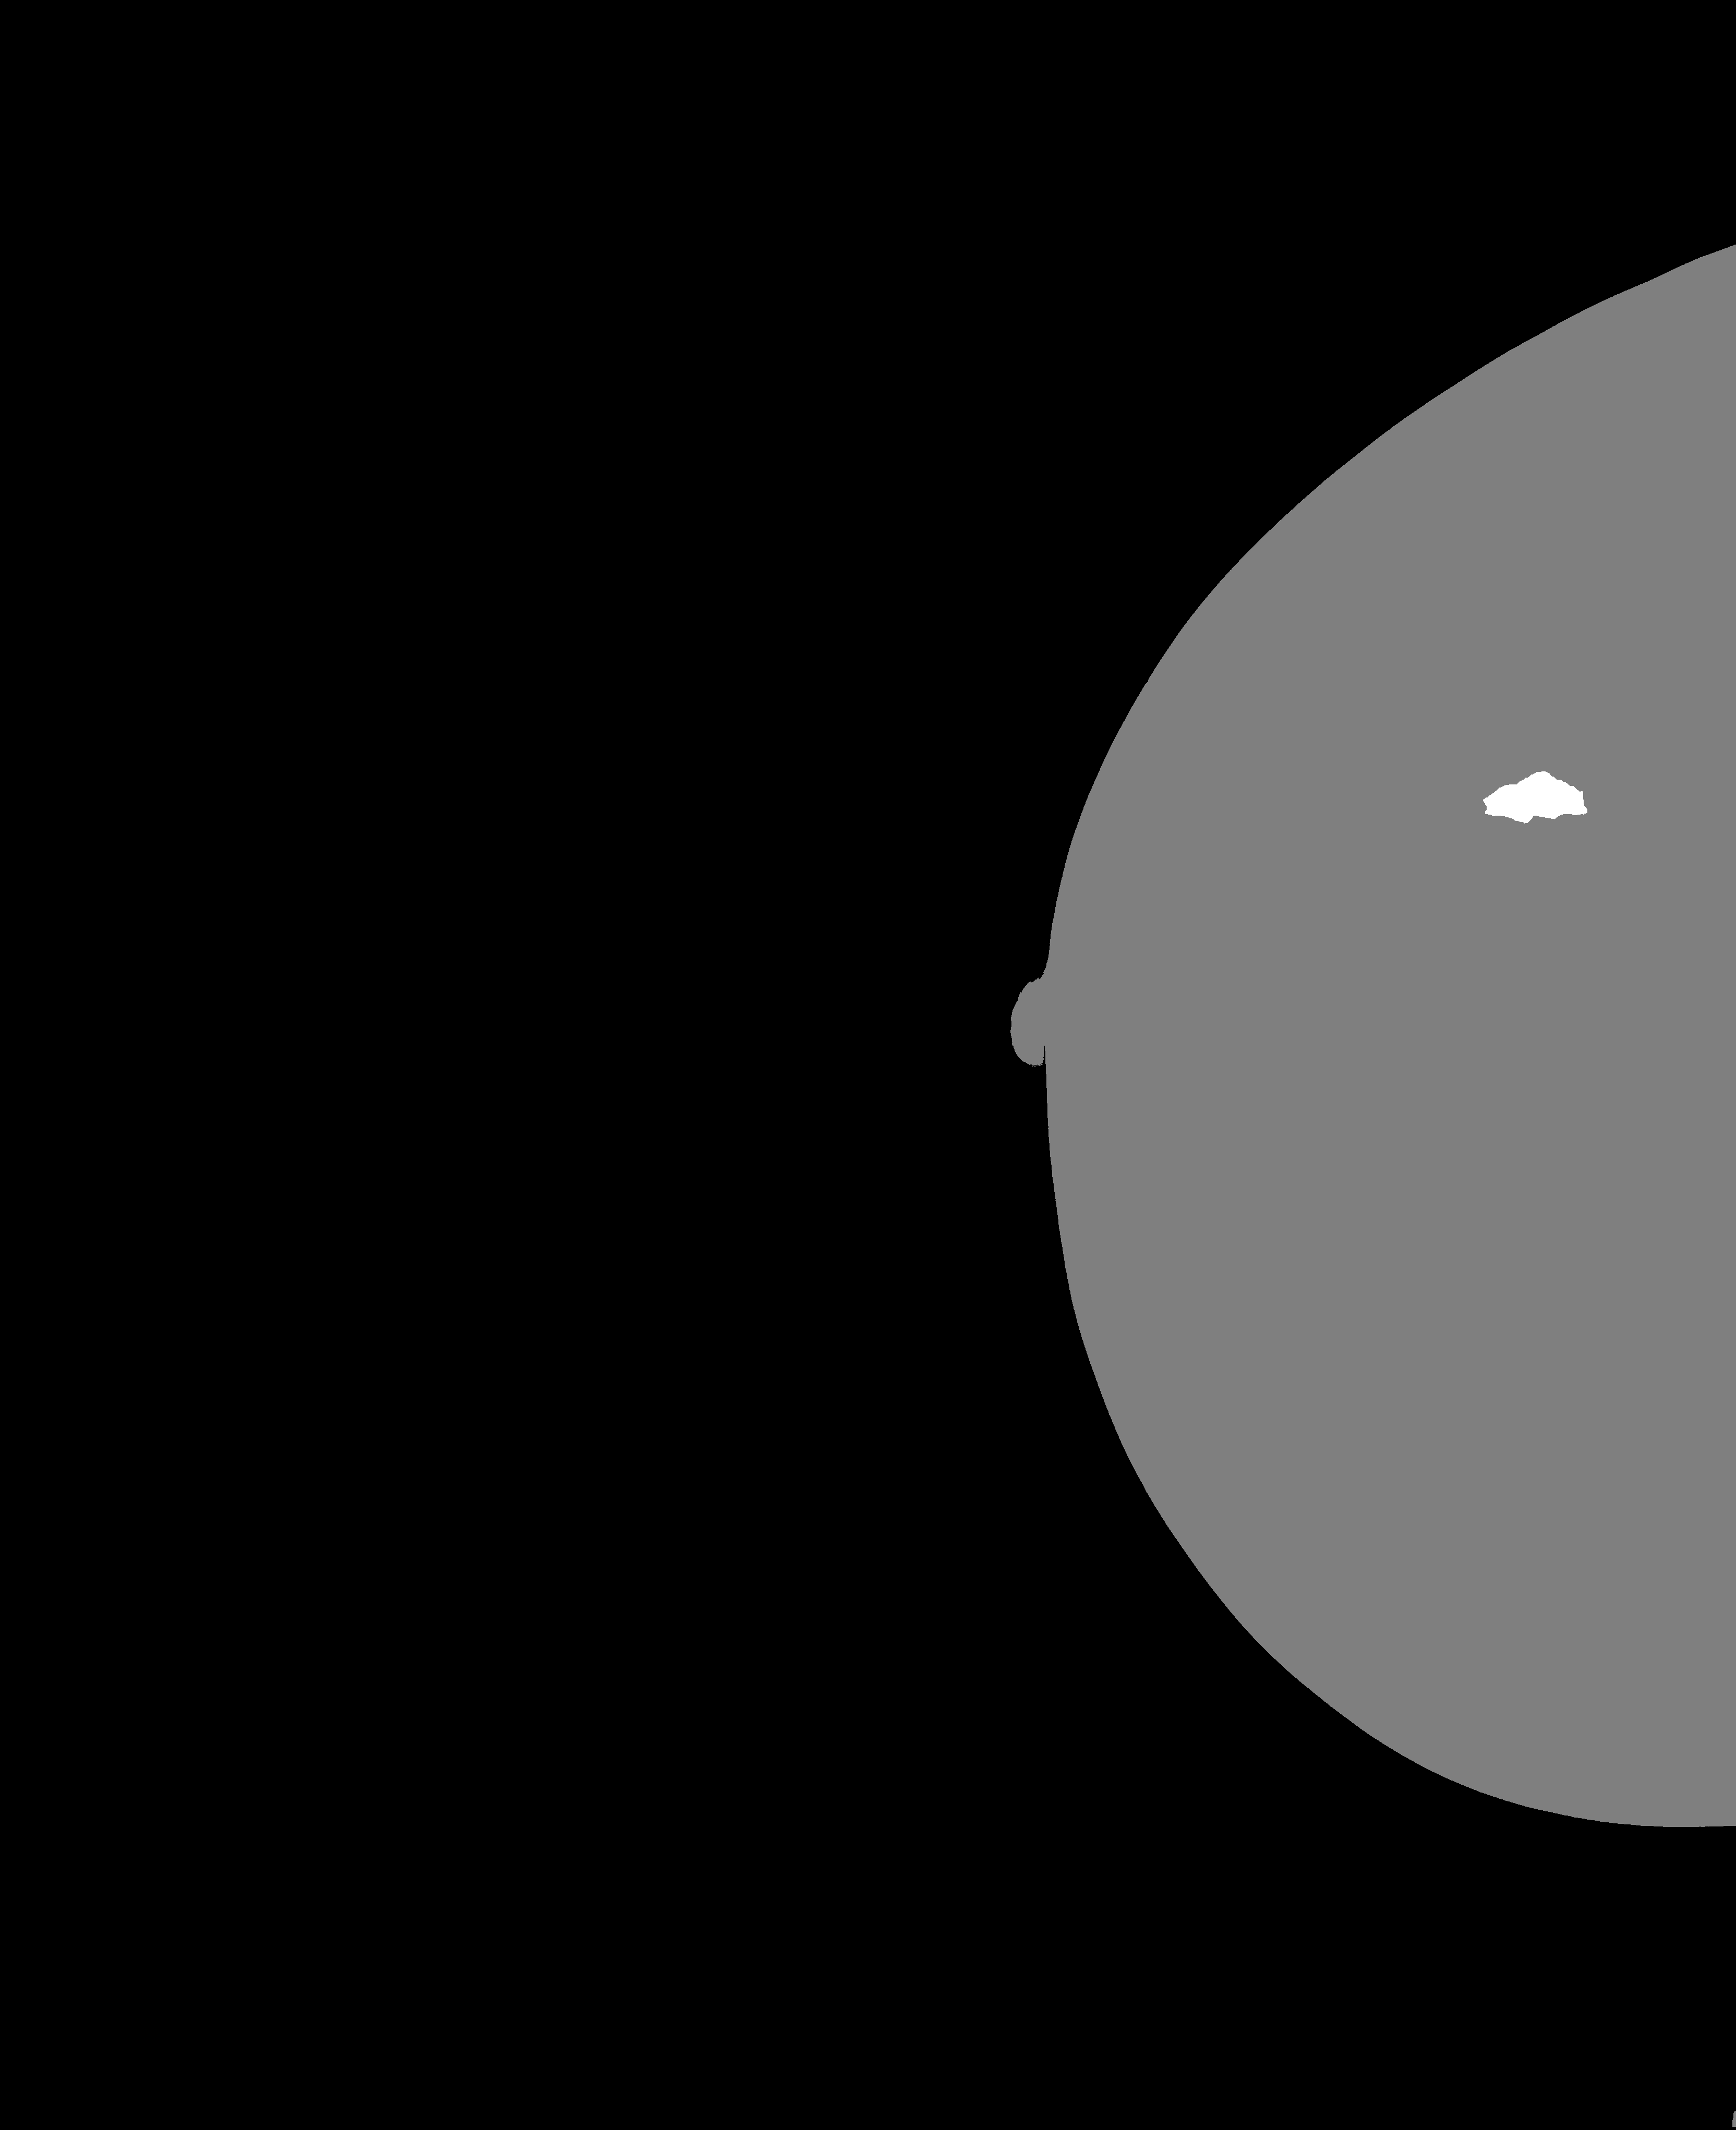
\includegraphics[height = 3.5cm]{plots/label_enhanced.png}
				\caption{Enhancement}
				\label{subfig:Preprocessingb}
			\end{subfigure}
			\begin{subfigure}{0.24\textwidth}
				\centering
					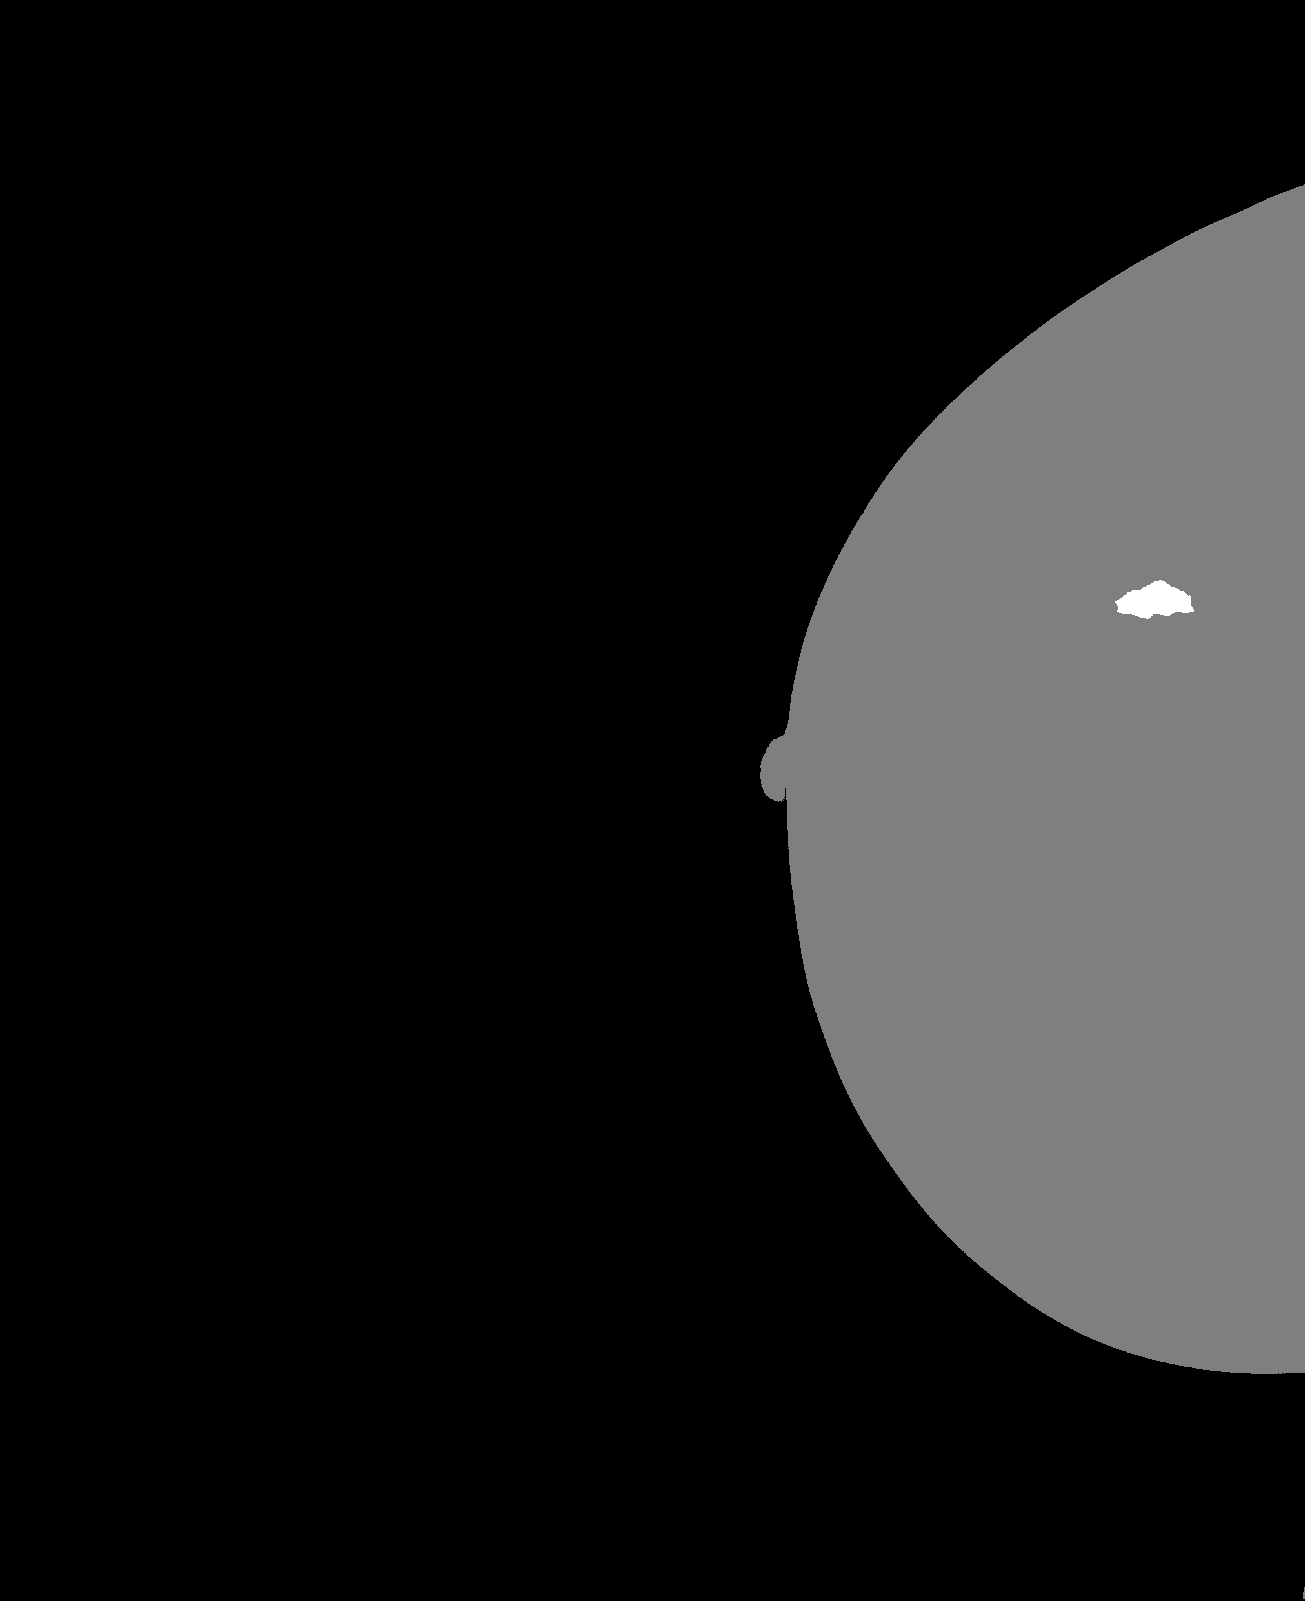
\includegraphics[height = 3.5cm]{plots/label_resized.png}
				\caption{Downsampling}
				\label{subfig:Preprocessingc}
			\end{subfigure}
			\begin{subfigure}{0.11\textwidth}
				\centering
					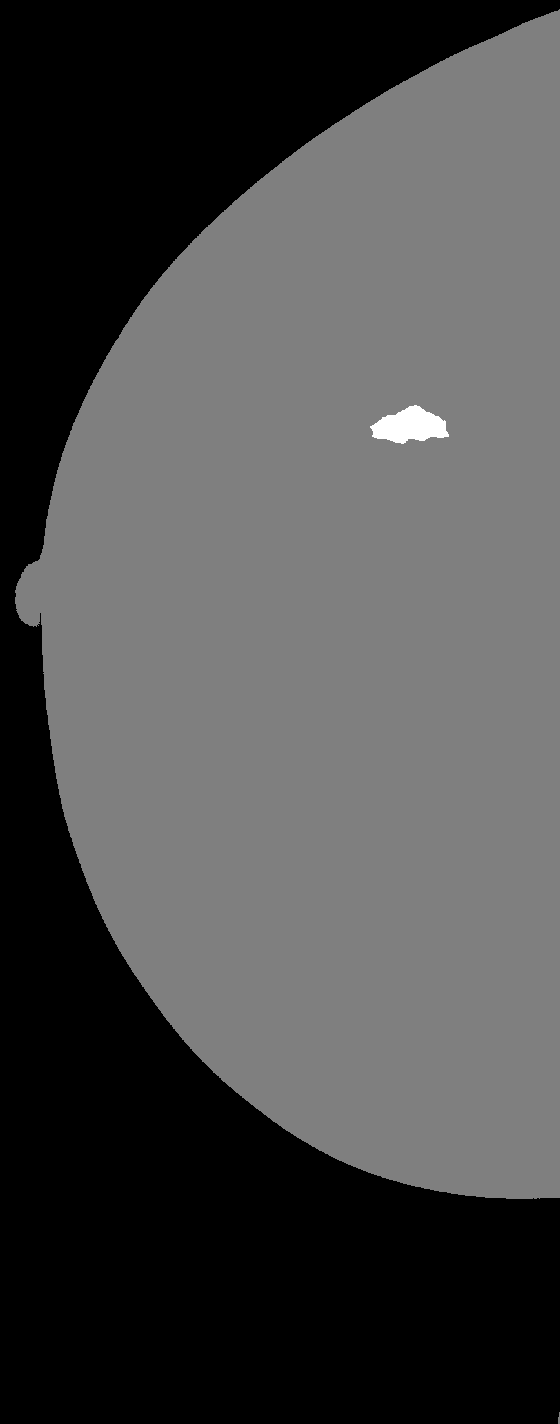
\includegraphics[height = 3.5cm]{plots/label_final.png}
				\caption{Final}
				\label{subfig:Preprocessingd}
			\end{subfigure}
			% img_108_146_1_RCC.png
		\end{figure}
	\end{frame}
	
	\begin{frame}
		\frametitle{Software}
		\begin{figure}
			\centering
			\begin{subfigure}{0.47\textwidth}
				\begin{subfigure}{\textwidth}
					
\includegraphics[width=\textwidth]{plots/tensorflow.png}
				\end{subfigure}
				\par \bigskip
				\begin{subfigure}{\textwidth}
					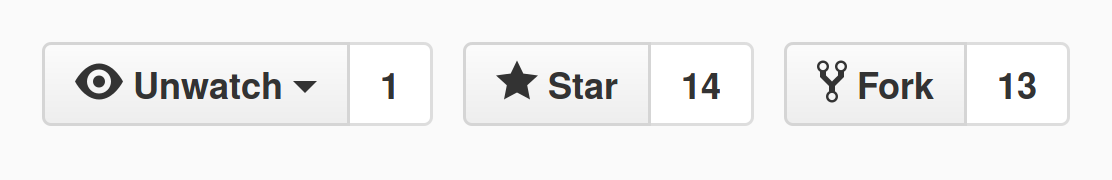
\includegraphics[width=\textwidth]{plots/github.png}
				\end{subfigure}
			\end{subfigure}
			~
			\begin{subfigure}{0.5\textwidth}
				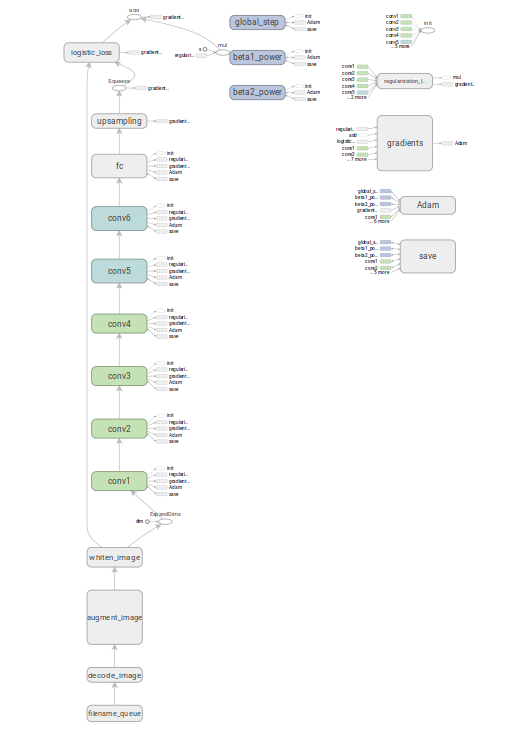
\includegraphics[width=\textwidth]{plots/tf_graph.png}
			\end{subfigure}
		\end{figure}
		%Seleccionar software, aprender tensorflow y havcer modelo.
	\end{frame}
	
	\begin{frame}
	    \frametitle{Overview of the solution}
		\begin{figure}
			\centering
			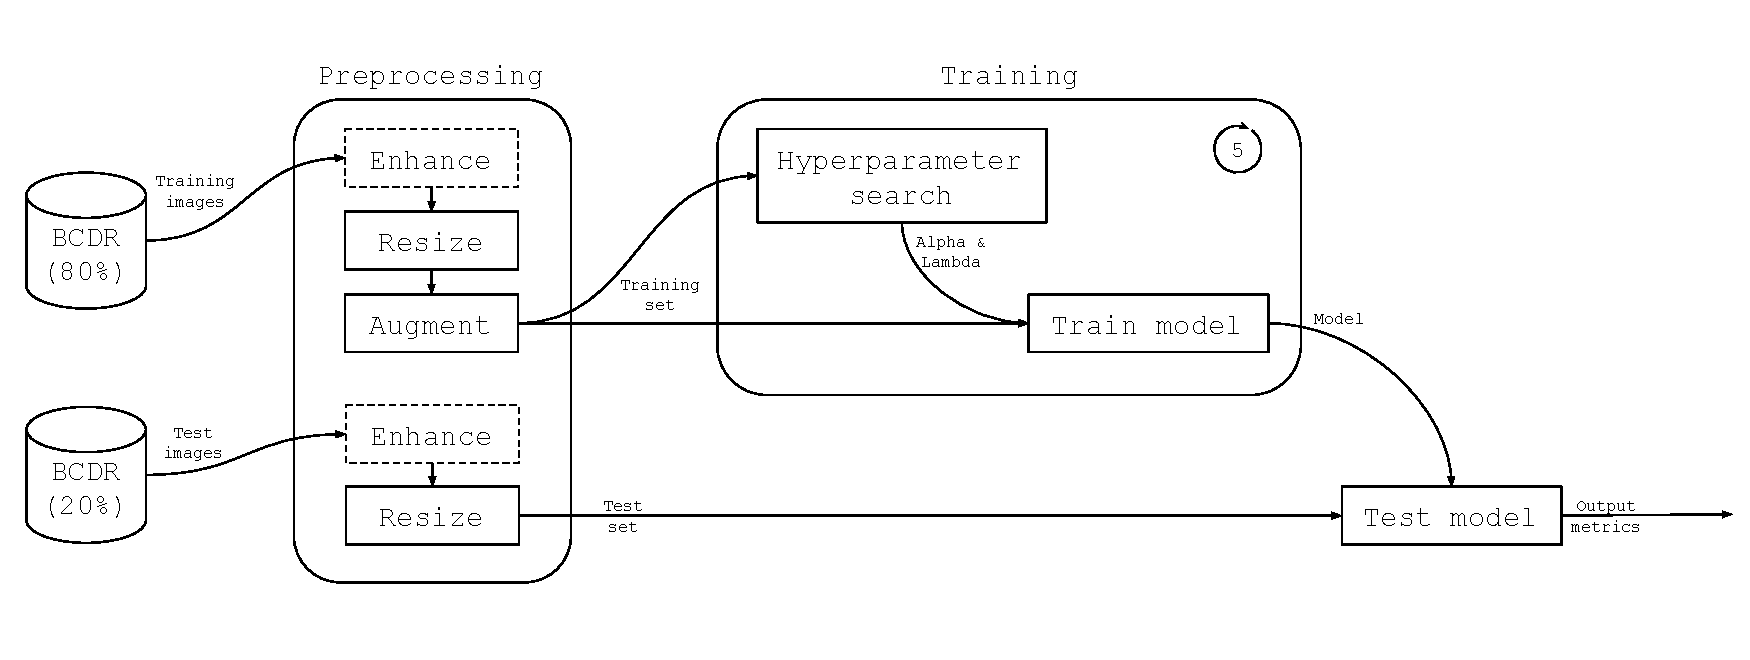
\includegraphics[width=\textwidth]{plots/overview.pdf}
		\end{figure}
	\end{frame}
	
	\begin{frame}
	    \frametitle{Model 1}
	    Simple architecture (206K parameters). Three configurations tested: no enhancement + no weighted loss, no enhancement + weighted loss and enhancement + weighted loss.
	    
	    \footnotesize
	    \begin{table}
	        \centering
	        \begin{tabular}{lcccccr}
	        \hline
	        \textbf{Layer} & \textbf{Filter} & \textbf{Stride} & \textbf{Pad} & \textbf{Dilation} & \textbf{Volume} & \textbf{Parameters} \\
	        \hline
	        \texttt{INPUT}	&- & -	& - & - & $52 \times 52 \times 1$ & -\\
	        \texttt{CONV -> RELU}	& $5 \times 5$ & 2 & 2 & 1 & $26 \times 26 \times 32$ & 832\\
	        \texttt{CONV -> RELU}	& $3 \times 3$ & 1 & 1 & 1 & $26 \times 26 \times 32$ & 9\,248\\
	        \texttt{CONV -> RELU}	& $3 \times 3$ & 2 & 1 & 1 & $13 \times 13 \times 64$ & 18\,496\\
	        \texttt{CONV -> RELU}	& $3 \times 3$ & 1 & 1 & 1 & $13 \times 13 \times 64$ & 36\,928\\
	        \texttt{CONV -> RELU}	& $3 \times 3$ & 1 & 2 & 2 & $13 \times 13 \times 96$ & 55\,392\\
	        \texttt{CONV -> RELU}	& $3 \times 3$ & 1 & 2 & 2 & $13 \times 13 \times 96$ & 83\,040\\
	        \texttt{CONV}			& $5 \times 5$ & 1 & 6 & 3 & $13 \times 13 \times 1$ & 2\,401\\
	        \texttt{BILINEAR (x4)}	& - & - && - & $52 \times 52 \times 1$ & -\\
	        \hline
	        \end{tabular}
        \end{table} % 206 337 params
	\end{frame}
	
	\begin{frame}
		\frametitle{Model 2}
		Modelled on a VGG network, winner of the 2014 ImageNet. Does not use dilation. Tested with no enhancement + weighted loss.
		% Say that it is like the Vgg-Net
		
		\footnotesize
		\begin{table}
			\centering
			\begin{tabular}{lccccr}
			\hline
			\textbf{Layer} & \textbf{Filter} & \textbf{Stride} &\textbf{Pad} & \textbf{Volume} & \textbf{Parameters} \\
			\hline
			\texttt{INPUT}	& -	& - & - & $112 \times 112 \times 1$ & -\\
			\texttt{CONV -> Leaky RELU} & $6 \times 6$ & 2 & 2 & $56 \times 56 \times 56$ & 2\,072\\
			\texttt{CONV -> Leaky RELU} & $3 \times 3$ & 1 & 1 & $56 \times 56 \times 56$ & 28\,280\\
			\texttt{MAXPOOL} & $2 \times 2$ & 2 & 0 & $28 \times 28 \times 56$ & -\\
			\texttt{CONV -> Leaky RELU} & $3 \times 3$ & 1 & 1 & $28 \times 28 \times 84$ & 42\,420\\
			\texttt{CONV -> Leaky RELU} & $3 \times 3$ & 1 & 1 & $28 \times 28 \times 84$ & 63\,588\\
			\texttt{MAXPOOL} & $2 \times 2$ & 2 & 0 & $14 \times 14 \times 84$ & -\\
			\texttt{CONV -> Leaky RELU} & $3 \times 3$ & 1 & 1 & $14 \times 14 \times 112$ & 84\,784\\
			\texttt{CONV -> Leaky RELU} & $3 \times 3$ & 1 & 1 & $14 \times 14 \times 112$ & 113\,008\\
			\texttt{CONV -> Leaky RELU} & $3 \times 3$ & 1 & 1 & $14 \times 14 \times 112$ & 113\,008\\
			\texttt{MAXPOOL} & $2 \times 2$ & 2 & 0 & $7 \times 7 \times 112$ & -\\
			\texttt{FC -> Leaky RELU} & $7 \times 7$ & 1 & 3 & $7 \times 7 \times 448$ & 2\,459\,072\\
			\texttt{FC} & $1 \times 1$ & 1 & 0 & $7 \times 7 \times 1$ & 449 \\
			\texttt{BILINEAR (x16)} & - & - & - & $112 \times 112 \times 1$ & -\\
			\hline
			\end{tabular}
		\end{table}
	\end{frame}
	
	\begin{frame}
		\frametitle{Model 3}
		Modelled on the Residual network, winner of the 2015 ImageNet. Deeper, fewer parameters and better resolution (4x). Tested with enhancement + weighted loss.
		
		\footnotesize
		\begin{table}
			\centering
			\begin{tabular}{lcccccr}
			\hline
			\textbf{Layer} & \textbf{Filter} & \textbf{Stride} & \textbf{Pad} & \textbf{Dilation} & \textbf{Volume} & \textbf{Parameters} \\
			\hline
			\texttt{INPUT}	&- & -	& - & - & $128 \times 128 \times 1$ & -\\
			\texttt{CONV -> LRELU}	& $6 \times 6$ & 2 & 2 & 1 & $64 \times 64 \times 32$ & 1\,184\\
			\texttt{CONV -> LRELU}	& $3 \times 3$ & 1 & 1 & 1 & $64 \times 64 \times 32$ & 9\,248\\
			\texttt{CONV -> LRELU}	& $3 \times 3$ & 2 & 1 & 1 & $32 \times 32 \times 64$ & 18\,496\\
			\texttt{CONV -> LRELU}	& $3 \times 3$ & 1 & 1 & 1 & $32 \times 32 \times 64$ & 36\,928\\
			\texttt{CONV -> LRELU}	& $3 \times 3$ & 1 & 2 & 2 & $32 \times 32 \times 128$ & 73\,856\\
			\texttt{CONV -> LRELU}	& $3 \times 3$ & 1 & 2 & 2 & $32 \times 32 \times 128$ & 147\,584\\
			\texttt{CONV -> LRELU}	& $3 \times 3$ & 1 & 2 & 2 & $32 \times 32 \times 128$ & 147\,584\\
			\texttt{CONV -> LRELU}	& $3 \times 3$ & 1 & 2 & 2 & $32 \times 32 \times 128$ & 147\,584\\
			\texttt{CONV -> LRELU}	& $3 \times 3$ & 1 & 4 & 4 & $32 \times 32 \times 256$ & 295\,168\\
			\texttt{CONV}	& $8 \times 8$ & 1 & 14 & 4 & $32 \times 32 \times 1$ & 16\,385\\
			\texttt{BILINEAR (x4)}		& - & - && - & $128 \times 128 \times 1$ & -\\
			\hline
			\end{tabular}
		\end{table}
	\end{frame}
	
	\begin{frame}
	    \frametitle{Training}
	    \textbf{Hyperparameter search:} 
	    For each fold, we train 20 networks with different learning rate and regularization parameters to select the best combination. We hold out 20\% of the training set for evaluation.
	    
	    \medskip
	    \textbf{Training:}	    
	    We trained the final models for 30 epochs using ADAM. Convergence was achieved.
	    
	    \medskip
	    \textbf{Evaluation:}
	    We use 5-fold cross-validation to generate our results and variability estimates.
	    
	\end{frame}

    \begin{frame}
        \frametitle{FROC curves}
           Free-response ROC curves plot the sensitivity of the system against the number of false predictions per image. Shading shows one standard error of the mean.
        \begin{figure}
	        \centering
		        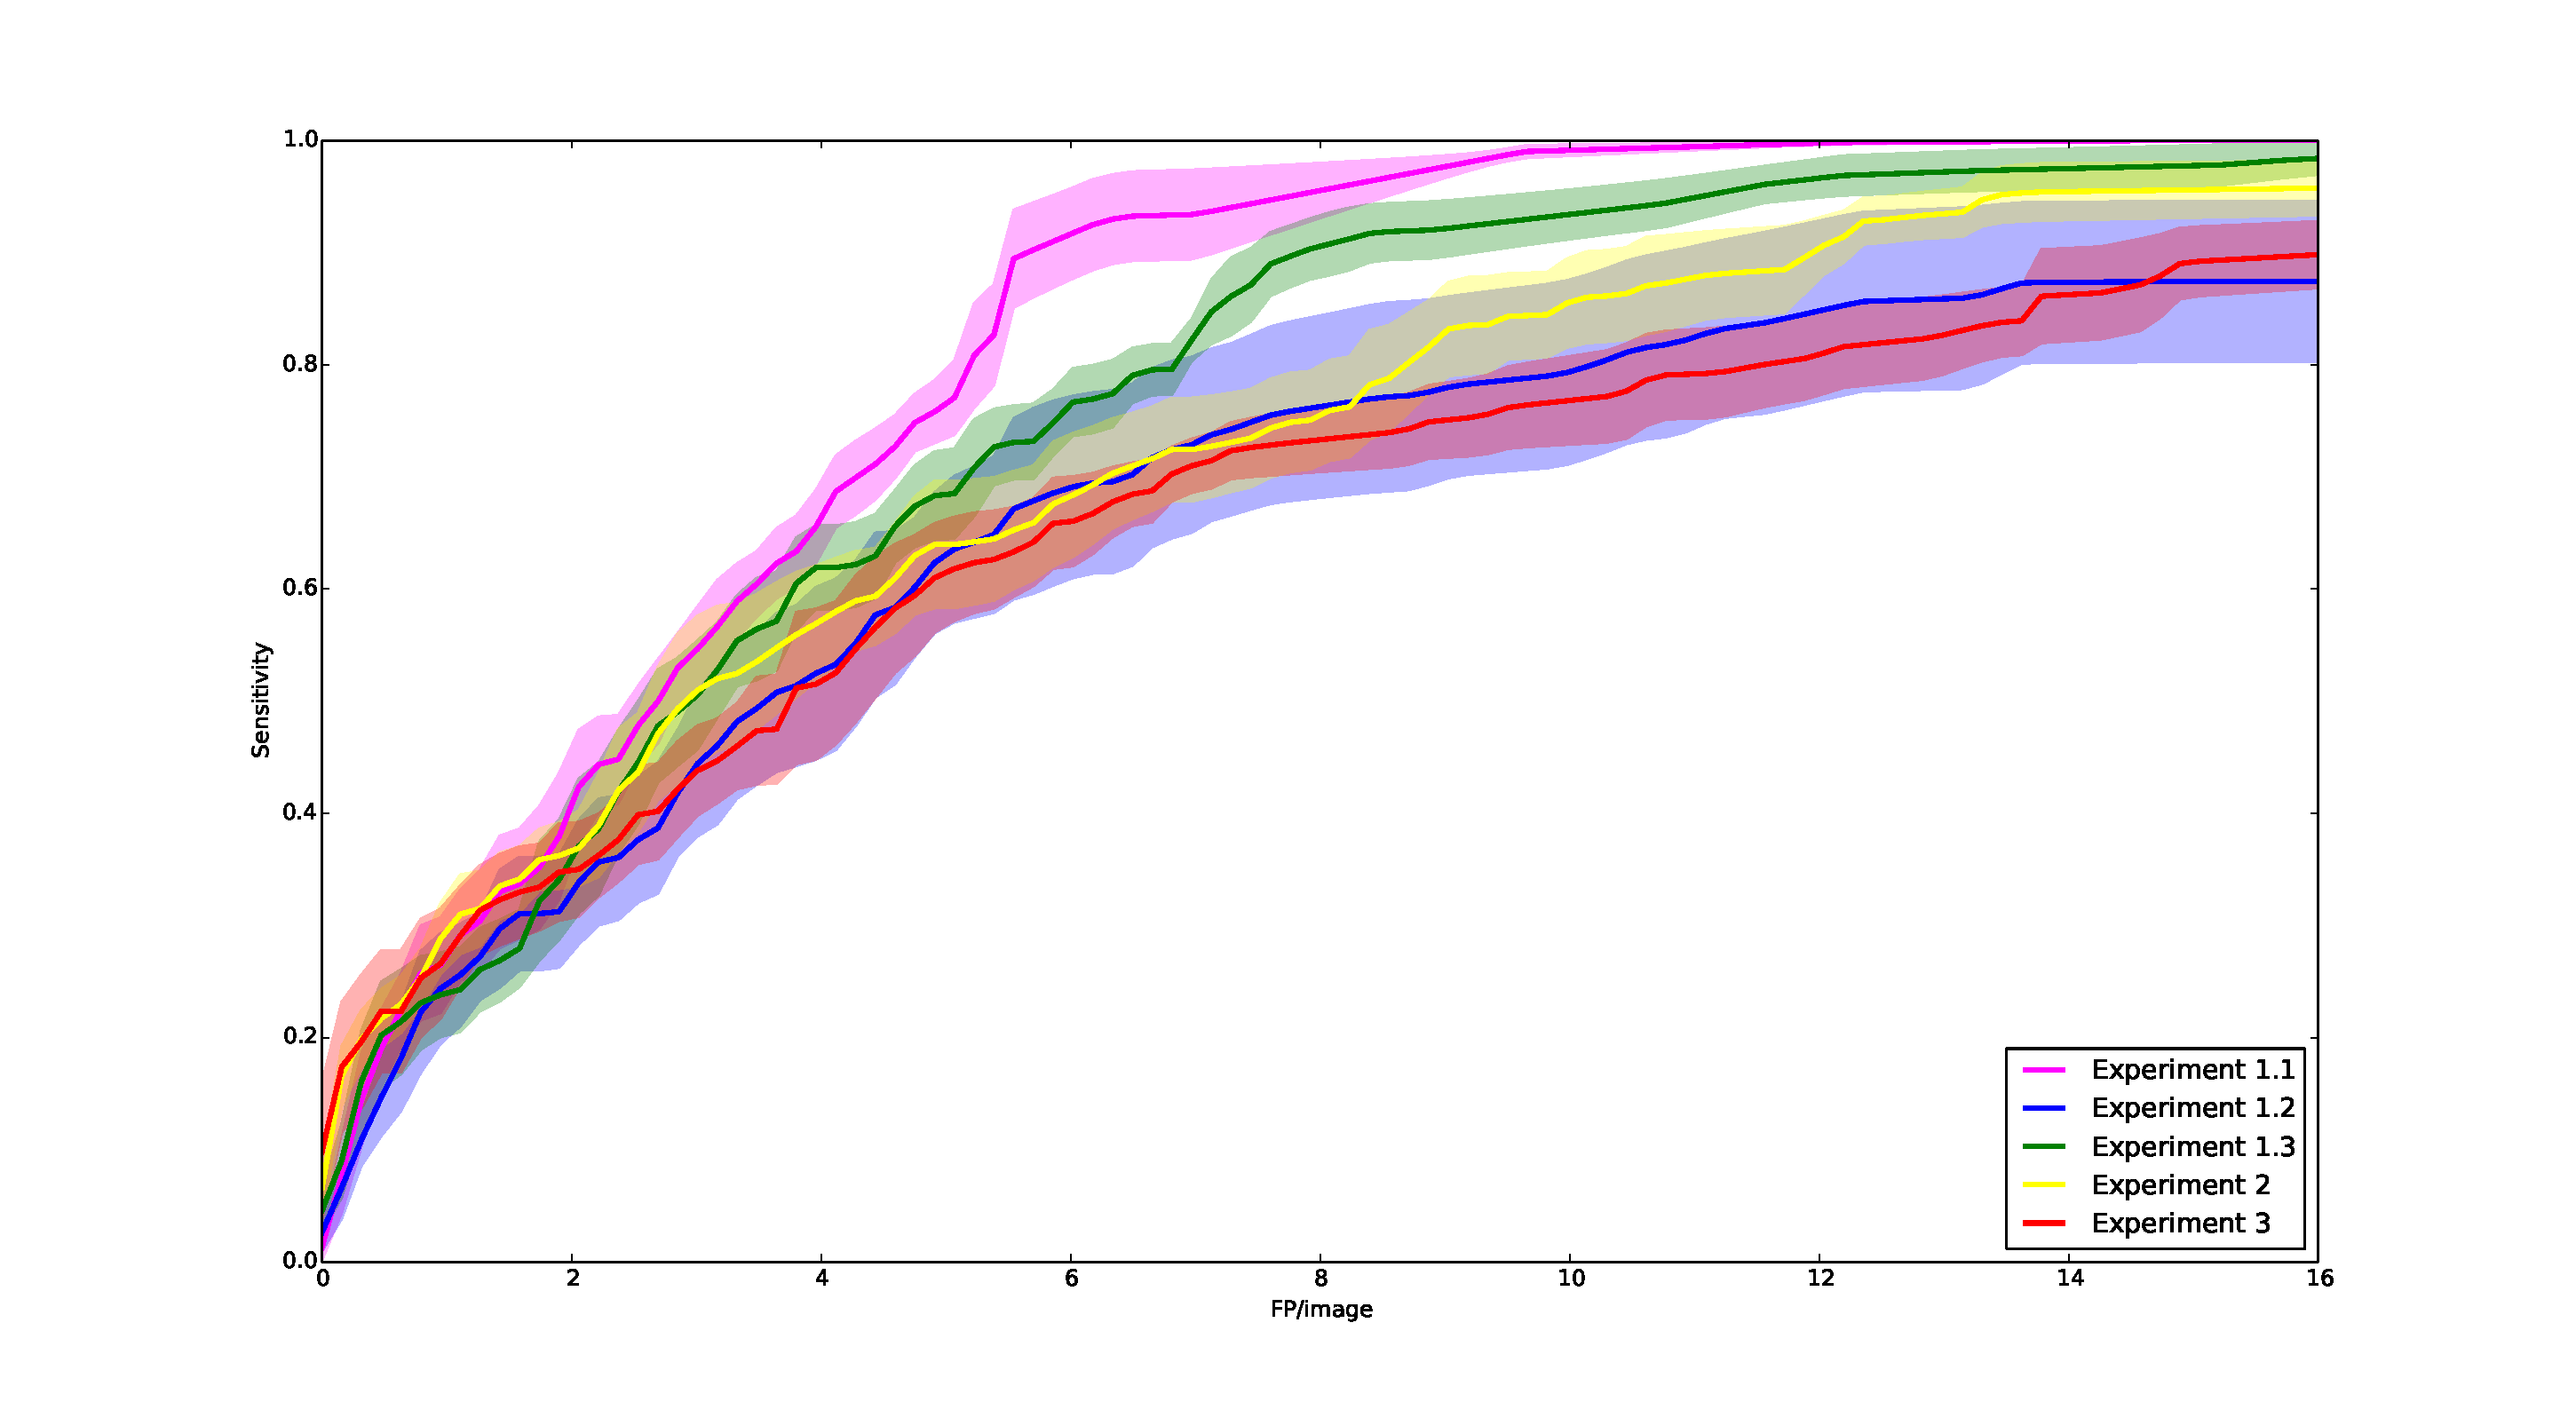
\includegraphics[width=\textwidth]{plots/FROC_plus_std.pdf}
        \end{figure}
    \end{frame}
    
    \begin{frame}
        \frametitle{IOU curves}
        Intersection-over-union as the threshold is varied. Each line is one fold.
        
        \begin{figure}
	        \centering
		        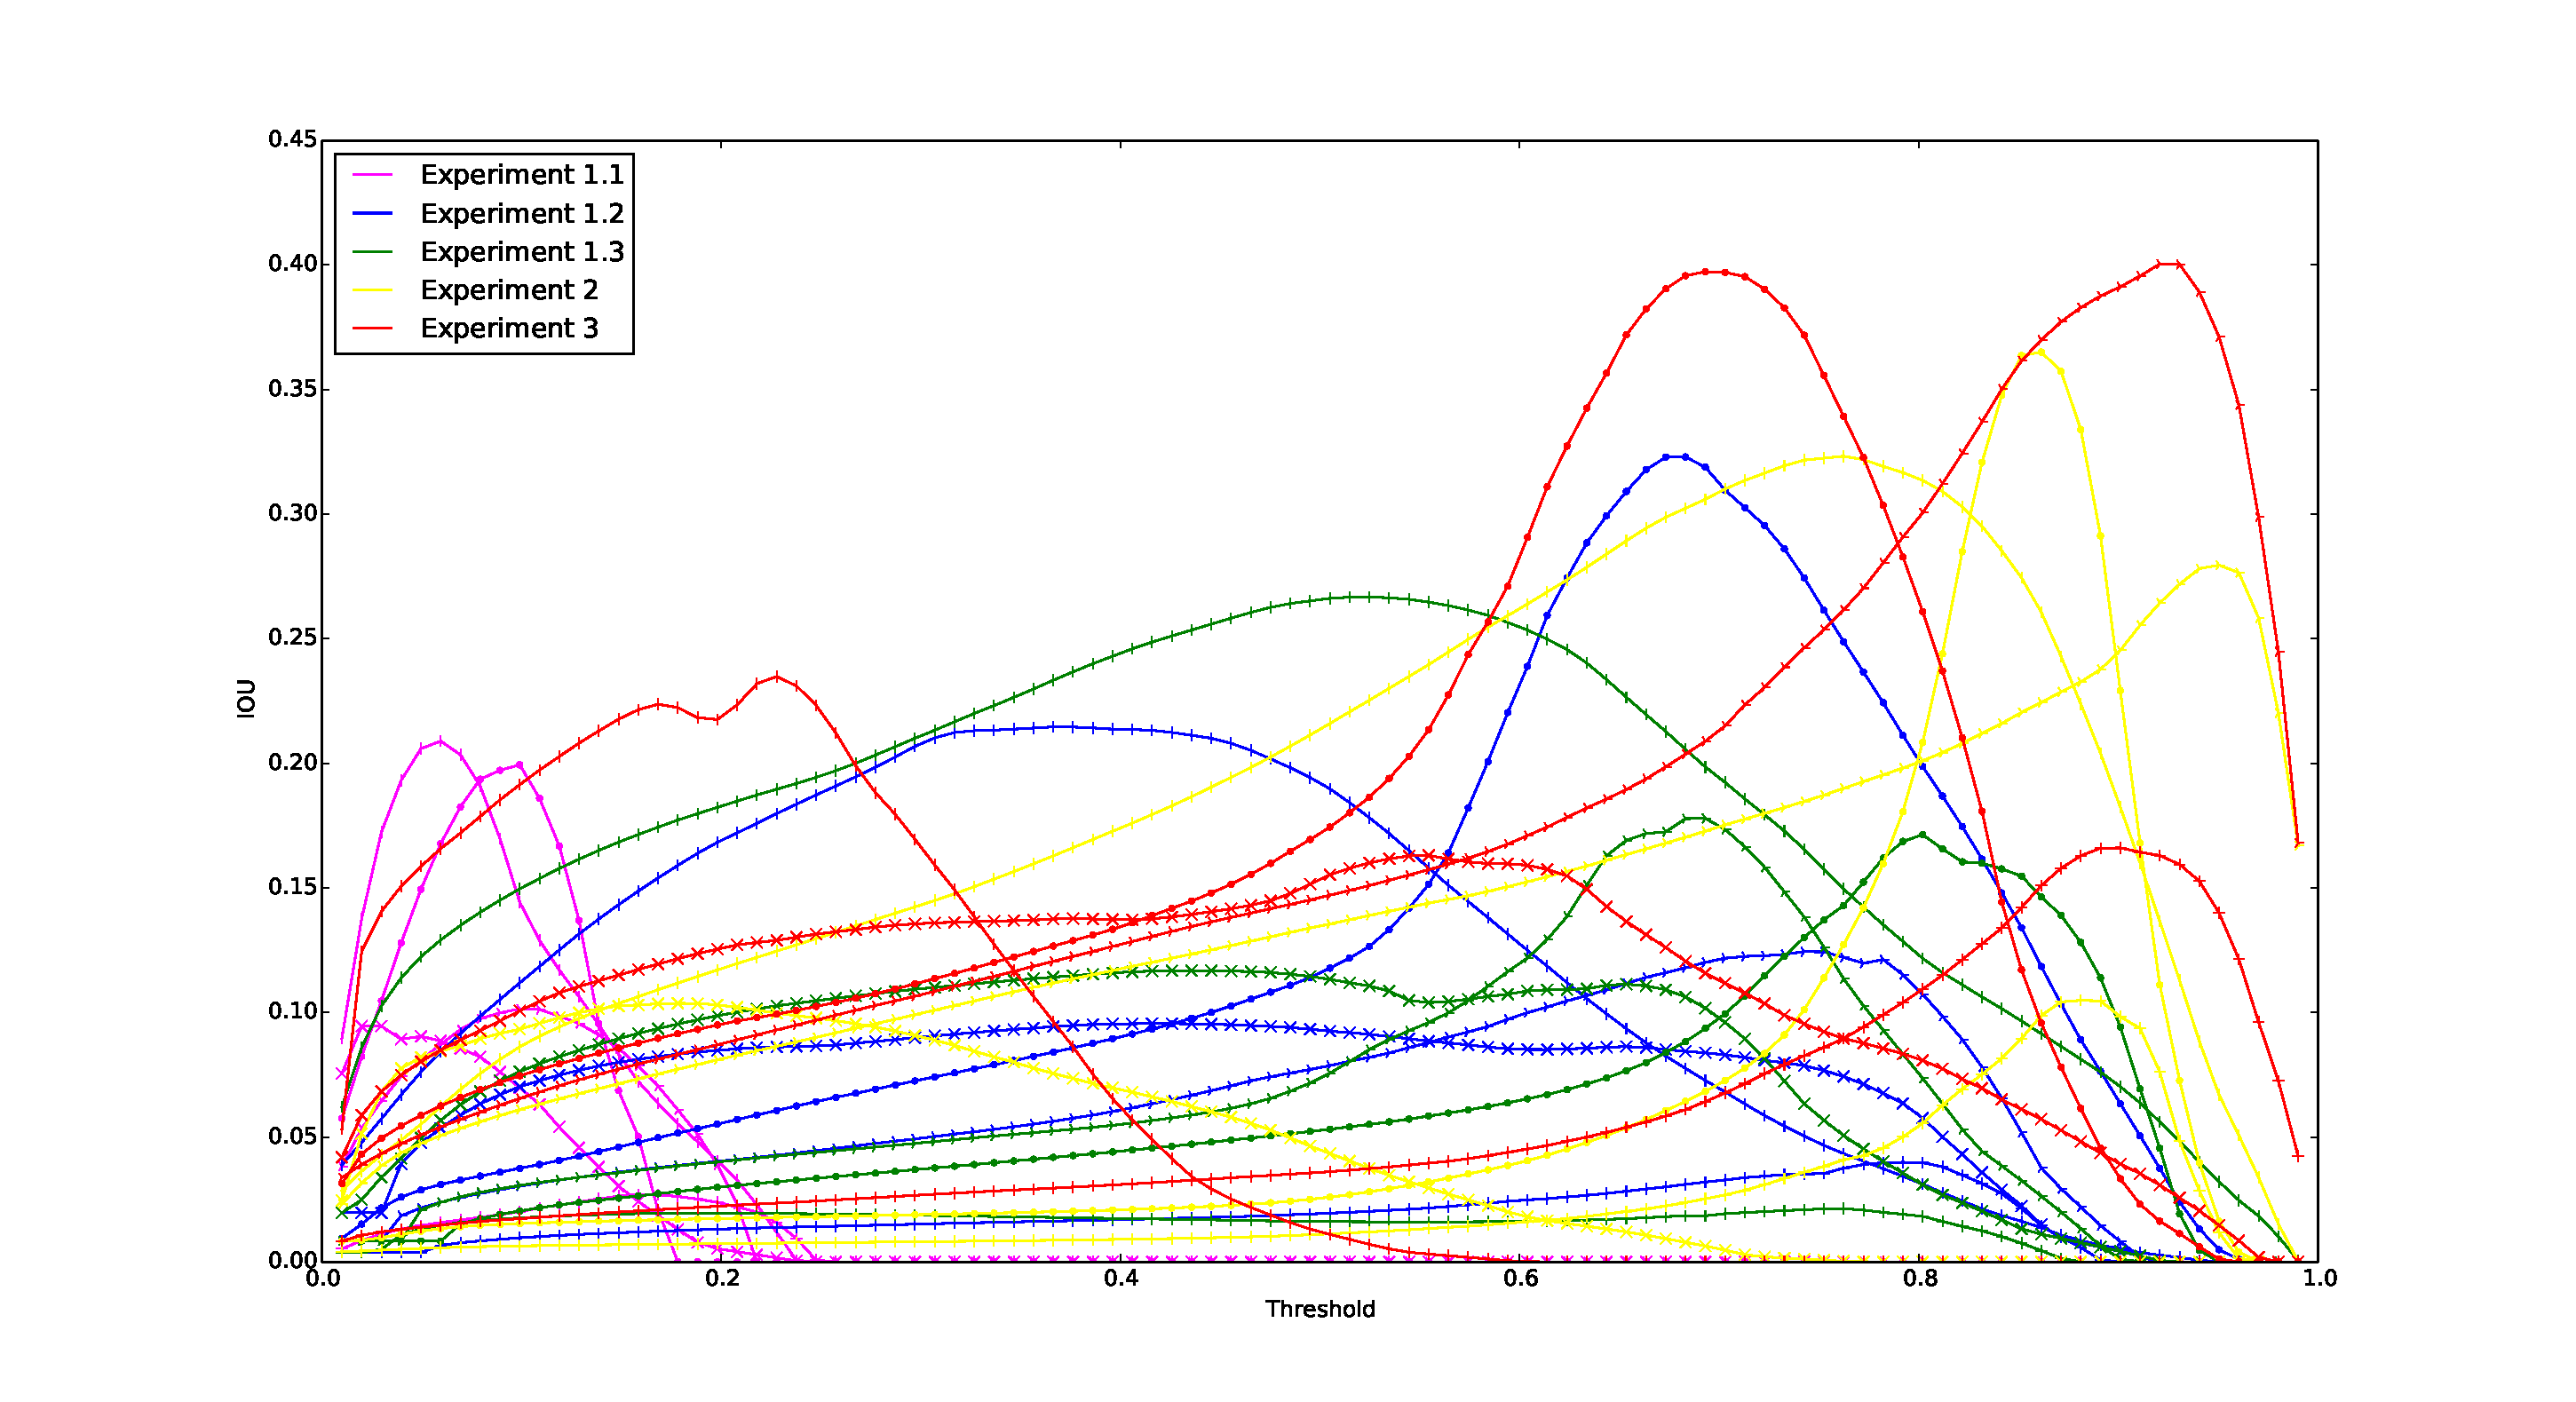
\includegraphics[width=\textwidth]{plots/IOU_all_folds.pdf}
        \end{figure}
    \end{frame}
    
    \begin{frame}
        \frametitle{Peak IOU}
        IOU value for the best threshold per fold.
        
        \footnotesize
        \begin{table}
	        \centering
	        \begin{tabular}{l*{6}{c}}
		        \hline
		         & \textbf{Fold 1} & \textbf{Fold 2} & \textbf{Fold 3} &\textbf{Fold 4} &\textbf{Fold 5} & \textbf{Average $\pm$ SEM} \\
		        \hline 
		        Experiment 1.1	&0.03	&0.09	&0.21	&0.20	&0.10	& $0.13 \pm 0.03$\\
		        Experiment 1.2	&0.04	&0.10	&0.21	&0.32	&0.12	& $0.16 \pm 0.04$\\
		        Experiment 1.3	&0.02	&0.12	&0.27	&0.17	&0.18	& $0.15 \pm 0.04$\\
		        Experiment 2	&0.11 	&0.10	&\textbf{0.32}	&0.37	& 0.28	& $0.24 \pm 0.05$\\
		        Experiment 3	&\textbf{0.17}	&\textbf{0.17}	&0.23	&\textbf{0.40}	&\textbf{0.40}	& $0.27 \pm 0.05$\\
		        Average			&0.07		&0.11	&0.25	&0.29	&0.22 &\\
		        \hline
	        \end{tabular}
        \end{table}
    \end{frame}
    
    
    \begin{frame}
        \frametitle{Qualitative results}  
        \begin{figure}
            \centering
            \begin{subfigure}{0.134\textwidth}
	            \centering
		            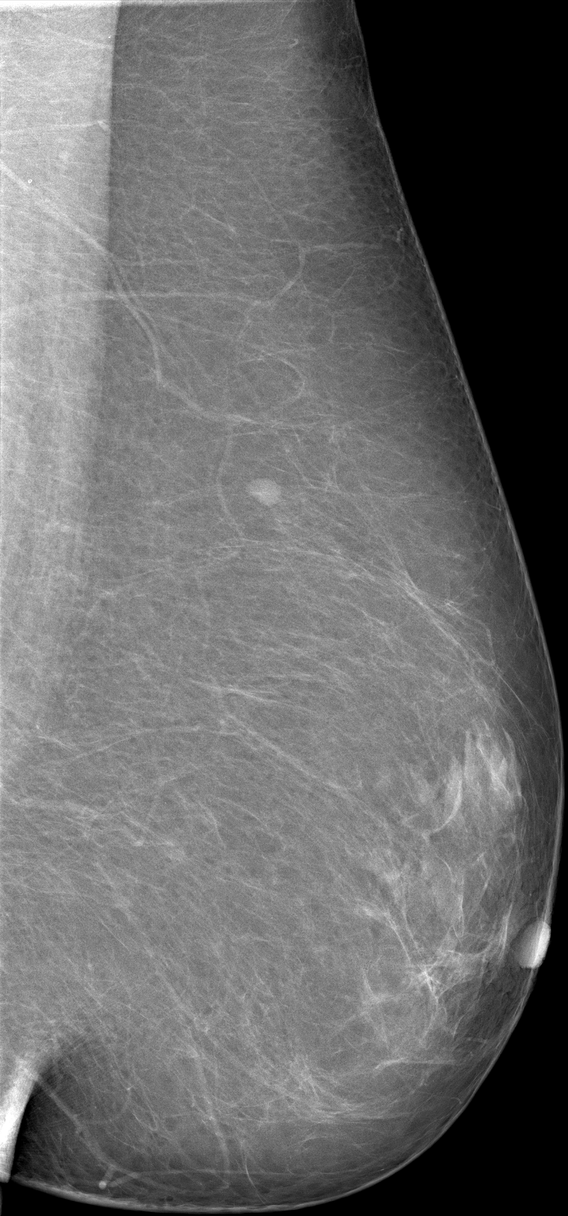
\includegraphics[width=\textwidth]{plots/examples/mammogram_1.png}
            \end{subfigure}
            \begin{subfigure}{0.134\textwidth}
	            \centering
		            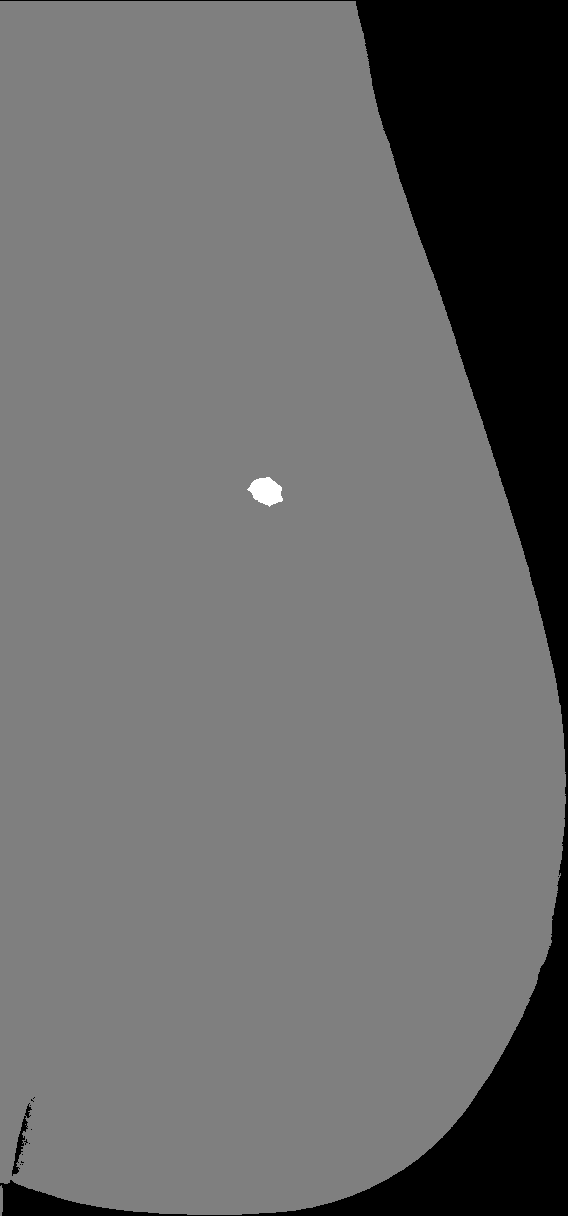
\includegraphics[width=\textwidth]{plots/examples/label_1.png}
            \end{subfigure}
            \begin{subfigure}{0.134\textwidth}
	            \centering
		            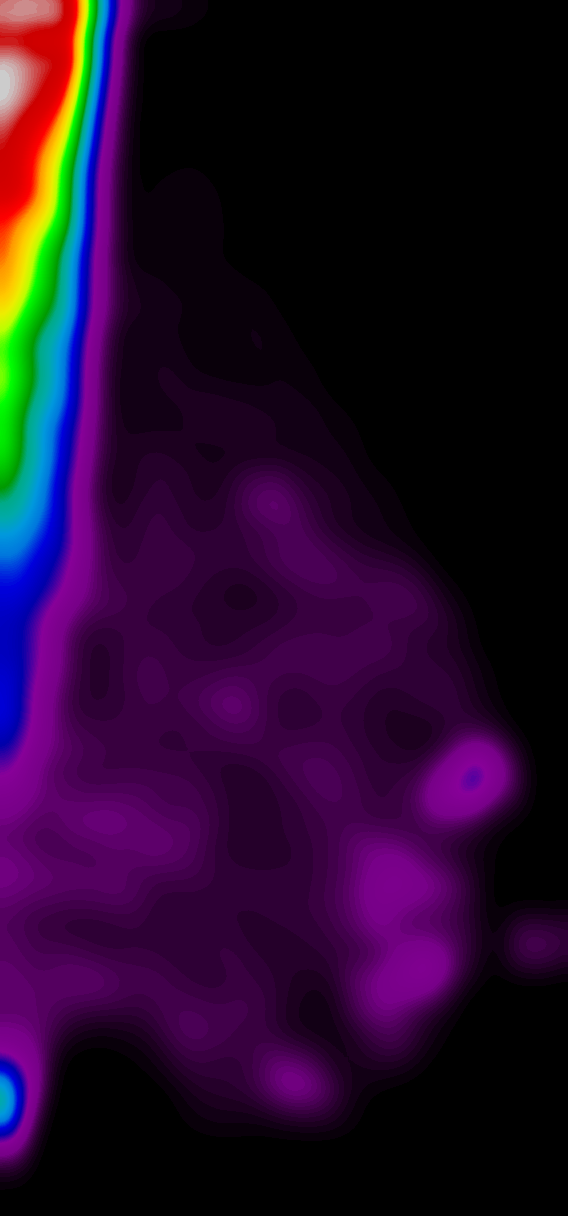
\includegraphics[width=\textwidth]{plots/examples/example1_probs_1_1.png}
            \end{subfigure}
            \begin{subfigure}{0.134\textwidth}
	            \centering
		            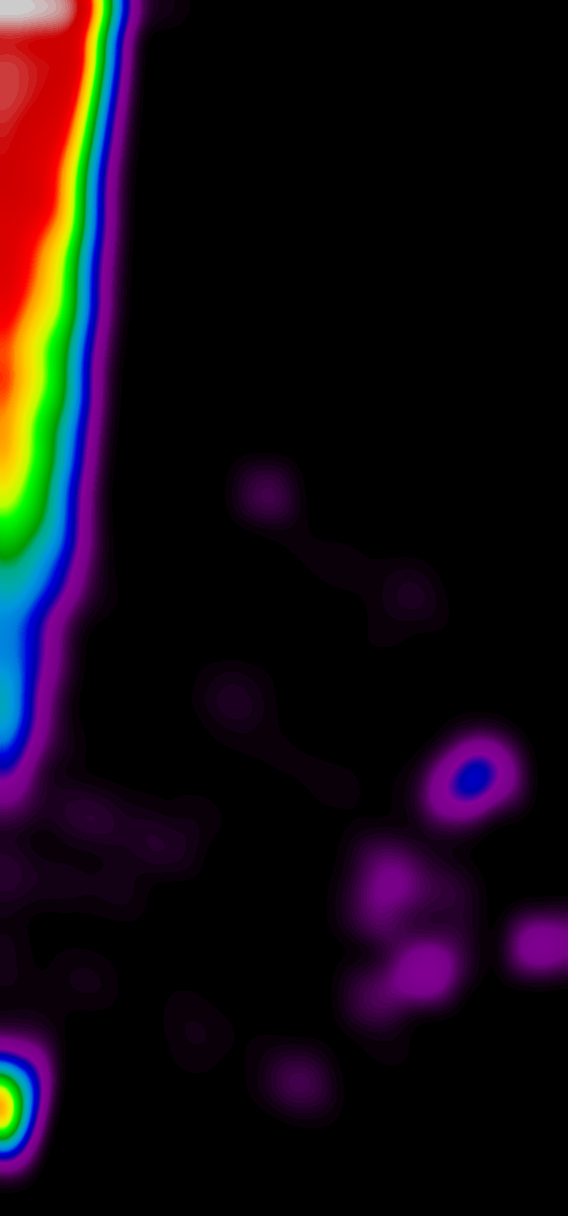
\includegraphics[width=\textwidth]{plots/examples/example1_probs_1_2.png}
            \end{subfigure}
            \begin{subfigure}{0.134\textwidth}
	            \centering
		            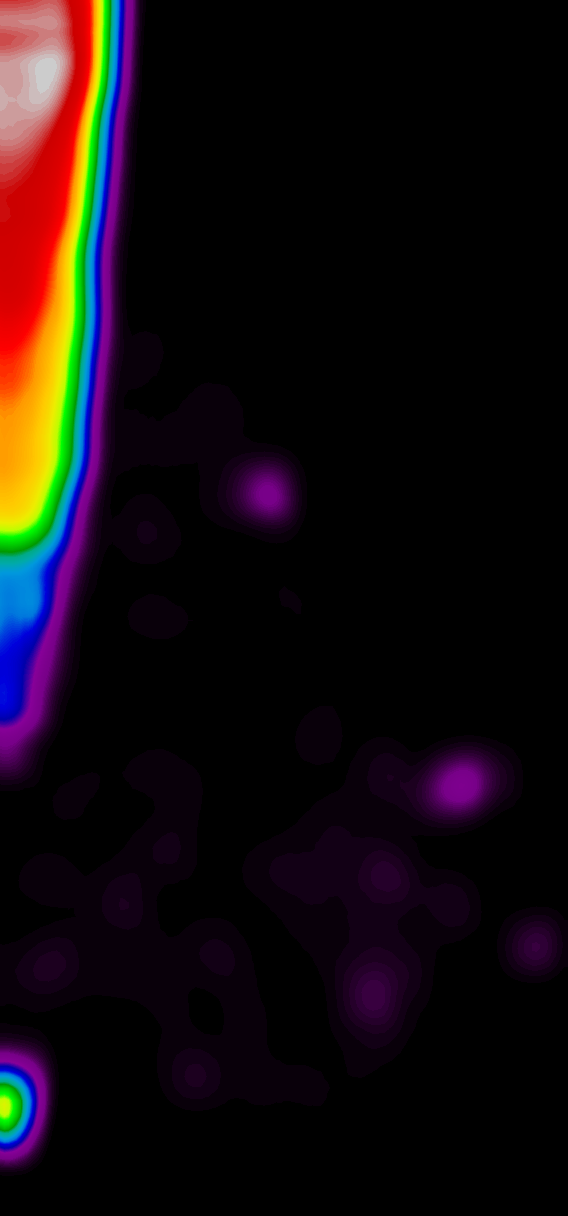
\includegraphics[width=\textwidth]{plots/examples/example1_probs_1_3.png}
            \end{subfigure}
            \begin{subfigure}{0.134\textwidth}
	            \centering
		            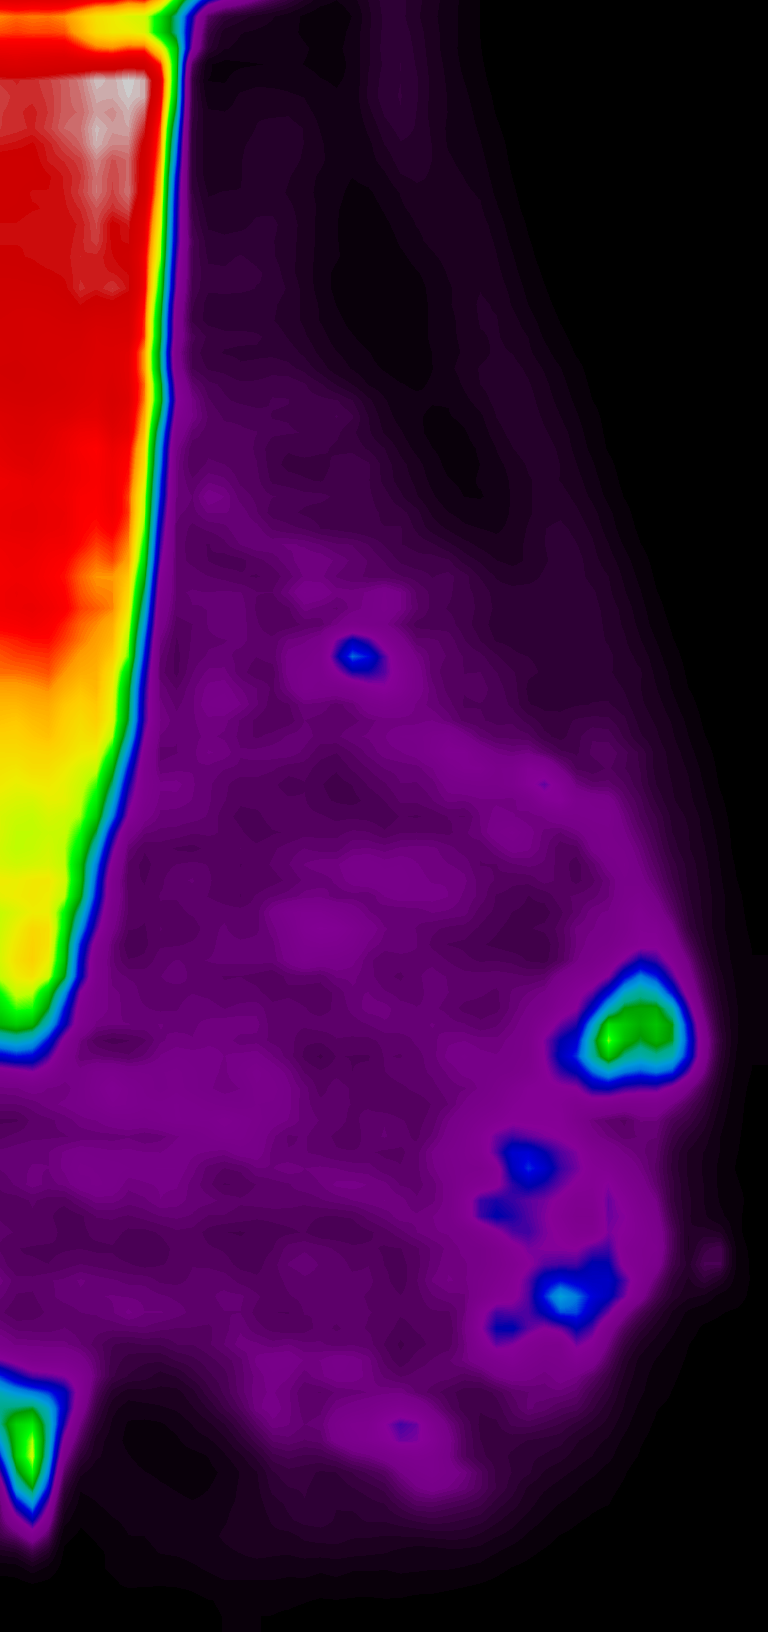
\includegraphics[width=\textwidth]{plots/examples/example1_probs_2.png}
            \end{subfigure}
            \begin{subfigure}{0.134\textwidth}
	            \centering
		            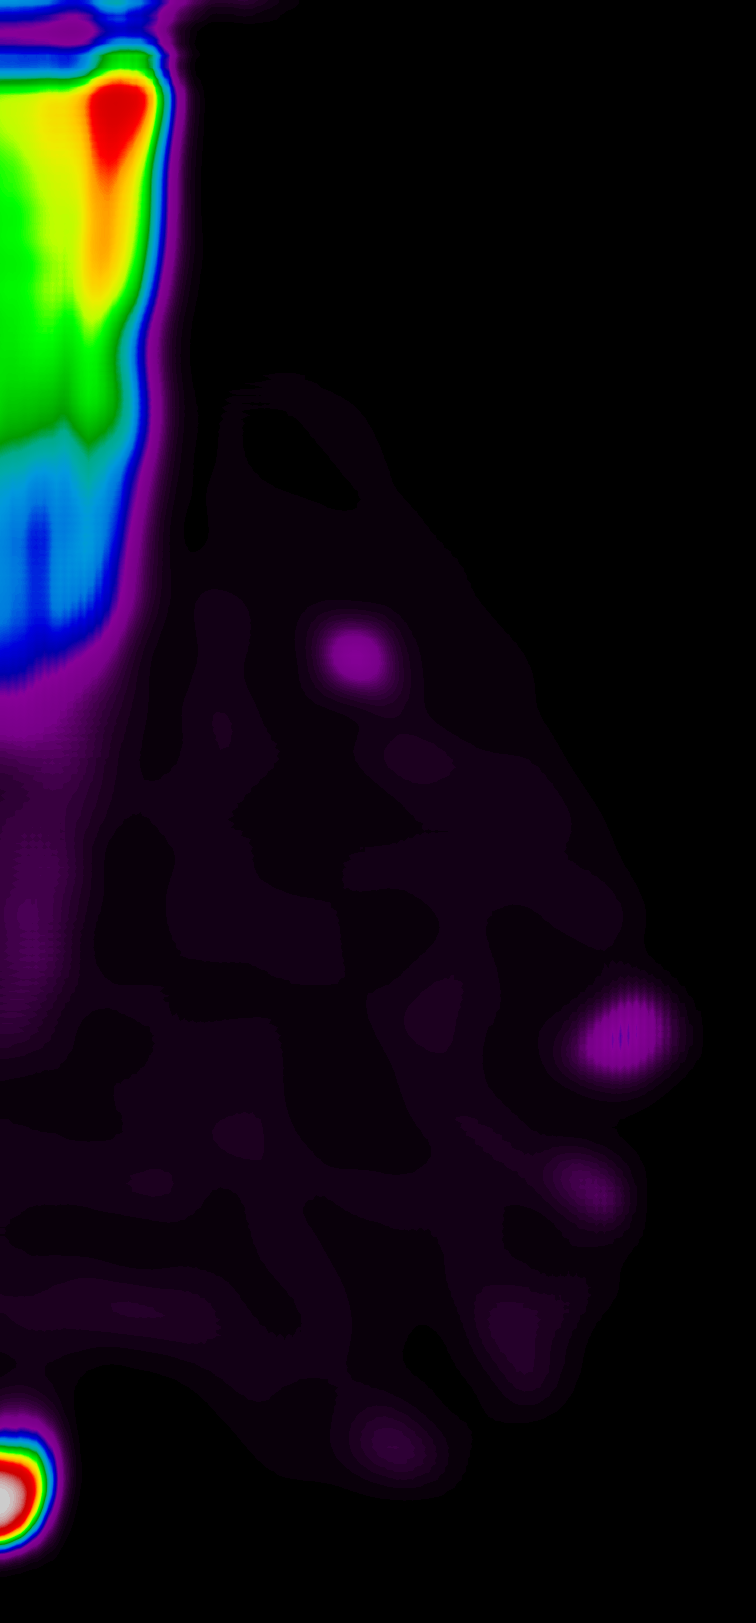
\includegraphics[width=\textwidth]{plots/examples/example1_probs_3.png}
            \end{subfigure}
            \\ \smallskip
            \begin{subfigure}{0.134\textwidth}
	            \centering
		            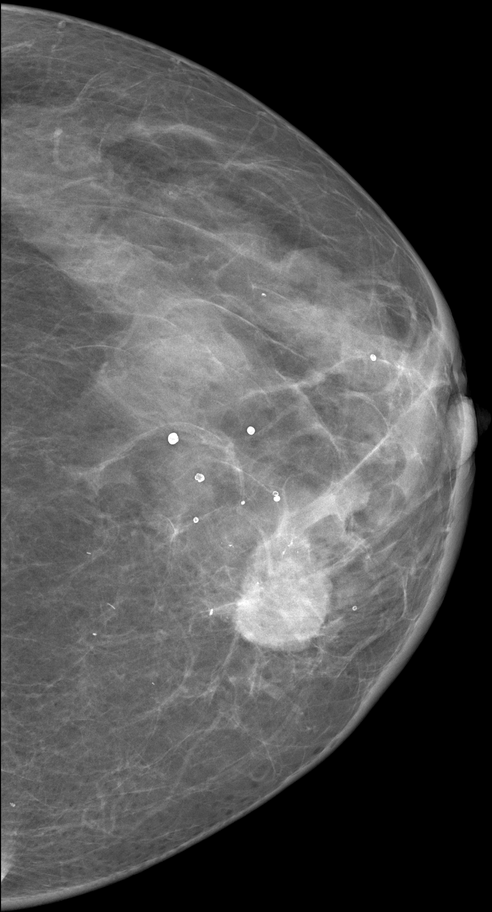
\includegraphics[width=\textwidth]{plots/examples/mammogram_5.png}
		        \caption*{\footnotesize Original}
            \end{subfigure}
            \begin{subfigure}{0.134\textwidth}
	            \centering
		            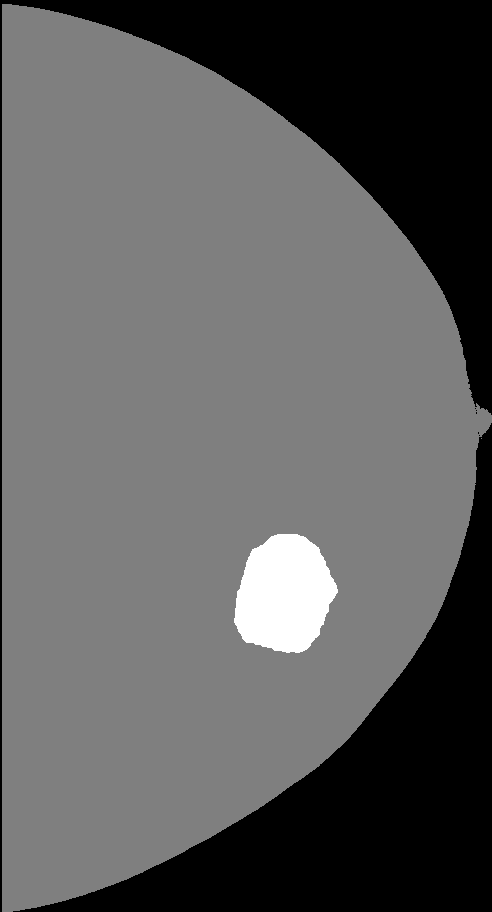
\includegraphics[width=\textwidth]{plots/examples/label_5.png}
		        \caption*{\footnotesize Label}
            \end{subfigure}
            \begin{subfigure}{0.134\textwidth}
	            \centering
		            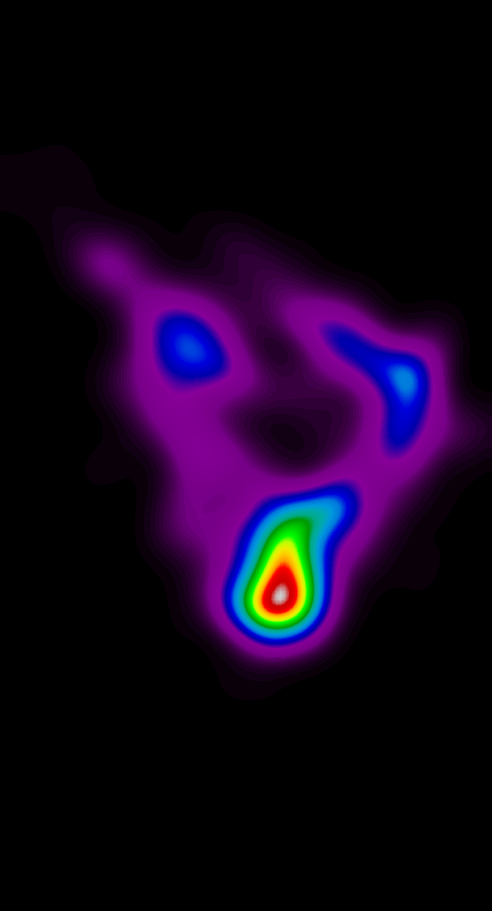
\includegraphics[width=\textwidth]{plots/examples/example5_probs_1_1.png}
	            \caption*{\footnotesize Exp. 1.1}
            \end{subfigure}
            \begin{subfigure}{0.134\textwidth}
	            \centering
		            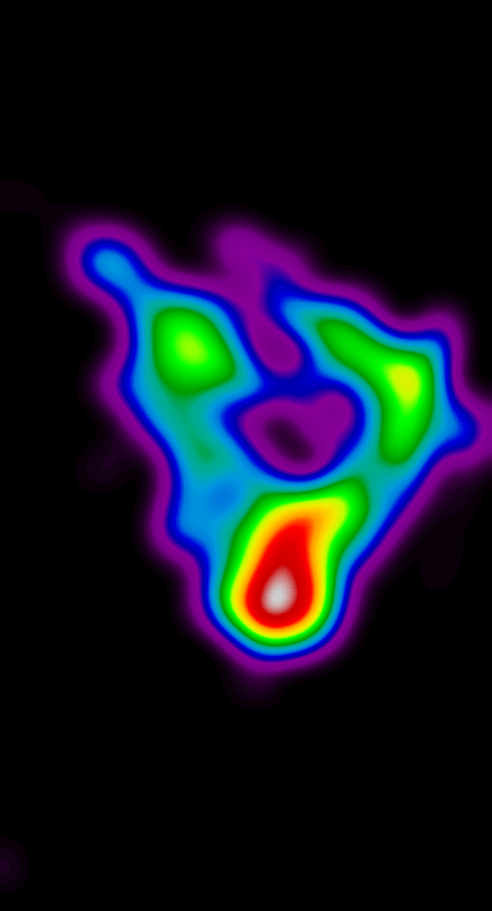
\includegraphics[width=\textwidth]{plots/examples/example5_probs_1_2.png}
	            \caption*{\footnotesize Exp. 1.2}
            \end{subfigure}
            \begin{subfigure}{0.134\textwidth}
	            \centering
		            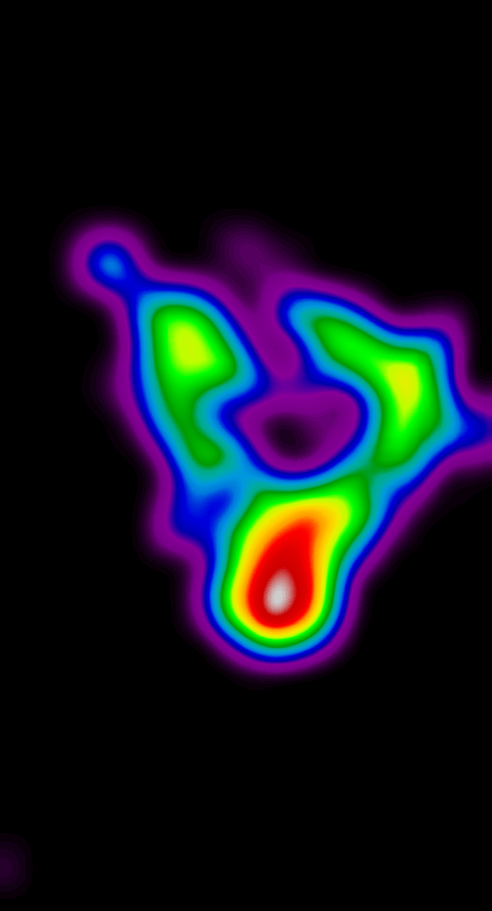
\includegraphics[width=\textwidth]{plots/examples/example5_probs_1_3.png}
	            \caption*{\footnotesize Exp. 1.3}
            \end{subfigure}
            \begin{subfigure}{0.134\textwidth}
	            \centering
		            \includegraphics[width=\textwidth]{plots/examples/example5_probs_2.png}
	            \caption*{\footnotesize Exp. 2}
            \end{subfigure}
            \begin{subfigure}{0.134\textwidth}
	            \centering
		            \includegraphics[width=\textwidth]{plots/examples/example5_probs_3.png}
	            \caption*{\footnotesize Exp. 3}
            \end{subfigure}
        \end{figure}
    \end{frame}
    
    \begin{frame}
        \frametitle{Qualitative results}
        \begin{figure}
            \centering
            \begin{subfigure}{0.134\textwidth}
	            \centering
		            \includegraphics[width=\textwidth]{plots/examples/mammogram_2.png}
            \end{subfigure}
            \begin{subfigure}{0.134\textwidth}
	            \centering
		            \includegraphics[width=\textwidth]{plots/examples/label_2.png}
            \end{subfigure}
            \begin{subfigure}{0.134\textwidth}
	            \centering
		            \includegraphics[width=\textwidth]{plots/examples/example2_probs_1_1.png}
            \end{subfigure}
            \begin{subfigure}{0.134\textwidth}
	            \centering
		            \includegraphics[width=\textwidth]{plots/examples/example2_probs_1_2.png}
            \end{subfigure}
            \begin{subfigure}{0.134\textwidth}
	            \centering
		            \includegraphics[width=\textwidth]{plots/examples/example2_probs_1_3.png}
            \end{subfigure}
            \begin{subfigure}{0.134\textwidth}
	            \centering
		            \includegraphics[width=\textwidth]{plots/examples/example2_probs_2.png}
            \end{subfigure}
            \begin{subfigure}{0.134\textwidth}
	            \centering
		            \includegraphics[width=\textwidth]{plots/examples/example2_probs_3.png}
            \end{subfigure}
            \\ \smallskip
            \begin{subfigure}{0.134\textwidth}
	            \centering
		            \includegraphics[width=\textwidth]{plots/examples/mammogram_4.png}
            \end{subfigure}
            \begin{subfigure}{0.134\textwidth}
	            \centering
		            \includegraphics[width=\textwidth]{plots/examples/label_4.png}
            \end{subfigure}
            \begin{subfigure}{0.134\textwidth}
	            \centering
		            \includegraphics[width=\textwidth]{plots/examples/example4_probs_1_1.png}
            \end{subfigure}
            \begin{subfigure}{0.134\textwidth}
	            \centering
		            \includegraphics[width=\textwidth]{plots/examples/example4_probs_1_2.png}
            \end{subfigure}
            \begin{subfigure}{0.134\textwidth}
	            \centering
		            \includegraphics[width=\textwidth]{plots/examples/example4_probs_1_3.png}
            \end{subfigure}
            \begin{subfigure}{0.134\textwidth}
	            \centering
		            \includegraphics[width=\textwidth]{plots/examples/example4_probs_2.png}
            \end{subfigure}
            \begin{subfigure}{0.134\textwidth}
	            \centering
		            \includegraphics[width=\textwidth]{plots/examples/example4_probs_3.png}
            \end{subfigure}
        \end{figure}
    \end{frame}

	\section[Conclusion]{Conclusion}
	\begin{frame}
		\frametitle{Conclusion}
		\begin{itemize}
			\item Convolutional networks can be used as an end-to-end trainable system to perform segmentation of mammograms.
			\item Small architectural variations are irrelevant as long as the architecture is flexible enough.
			\item Using a weighted loss function improves performance whereas enhancement helps only slightly.
			\item Hyperparameter fine-tuning is necessary to find a good minimum.
			\item The bottleneck for learning seems to be the small data sets.
			%\item Advances in segmentation of real-life images translate to mammographic images.
			\item Training small-to-medium networks is feasible with the available resources.
			\item Convolutional networks remain a promising option for future medical imaging research.
		\end{itemize}
	\end{frame}
	
	\begin{frame}
	    \frametitle{Contributions}
	    \begin{itemize}
	        \item First reported use of convolutional networks for breast cancer lesion segmentation.
	        \item Small, modern architectures tailored to segmentation. 
	        \item Mammographic data set and preprocessing tools.
	        \item Software for designing, training and evaluating convolutional networks.
	        \item Support to other deep learning projects in the campus.
	    \end{itemize}
	\end{frame}
	
	\begin{frame}
		\frametitle{Future work}
		\begin{itemize}
		    \item Create a high-quality, large data set.
		    \item Curate data by deleting obvious lesions, benign lesions and chest muscle, labelling other kind of lesions and breast tissue or joining images from different sources.
		    \item Validate results using different architectures and bigger data sets.
		    \item Use standard computer vision features as input to the network.
		    \item Incorporate current trends to newer architectures.
		    \item Develop standard evaluation metrics for these kind of predictions.
		\end{itemize}
	\end{frame}

	\begin{frame}[c]
		\begin{center}
			\begin{figure}
				\includegraphics[width=0.25\textwidth]{plots/questions.png}
			\end{figure}
		\end{center}
	\end{frame}

\end{document}
